
\chapter{Le dispositif expérimental} \label{chap:chap3}

\begin{fmffile}{chapitre3}

La particule élémentaire la plus massive du Modèle Standard est le quark top, avec une masse d'environ \SI{173}{\GeV}. Inexistant à l'état stable dans la nature, il est nécessaire de le produire pour l'étudier. Pour cela, il faut être en mesure de générer des particules beaucoup plus énergétiques. La stratégie consiste à utiliser des accélérateurs qui permettent de collisionner des particules à grande énergie et ainsi de produire de nouvelles particules issues de la collision.

On distingue deux grandes classes d'accélérateurs de particules:
\begin{description}
  \item [Les accélérateurs circulaires]
  \begin{sloppypar}
   Dans ces dispositifs les particules sont accélérées le long d'un anneau. En permettant de nombreuses rotations, les particules peuvent atteindre de très hautes énergies. Cependant, lors d'une rotation, les particules chargées sont soumises à l'effet synchrotron. Il s'agit d'un rayonnement dont la valeur est inversement proportionnelle à $rm^4$ avec $r$ le rayon de  courbure et $m$ la masse de la particule accélérée. Autrement dit, plus le rayon de courbure et la masse sont élevés, moins le rayonnement synchrotron amputera de l'énergie aux particules à collisionner. Cela implique l'utilisation de particules lourdes comme des protons si l'on souhaite minimiser les pertes d'énergie. Les protons n'étant pas élémentaires, leurs structure interne va générer lors d'une collision plusieurs phénomènes parasites impactant la précision des mesures.
  \end{sloppypar}
    \item [Les accélérateurs linéaires] 
    \begin{sloppypar}
      Comme leur nom l'indique, ils accélèrent les particules en ligne droite. Due à la trajectoire finie des particules accélérées, l'énergie à la collision est limitée. Cependant, l'absence de rayonnement synchrotron permet d'utiliser des particules élémentaires de basse masse. En utilisant des particules comme l'électron, on assure des signatures extrêmement claires dans le détecteur, ce qui permet d'effectuer des mesures de précision.
    \end{sloppypar}
\end{description}


Le LHC (\emph{Large Hadron Collider}) \cite{LHC} est un collisionneur circulaire \Pproton{}-\Pproton{}. Il est donc un excellent dispositif pour pouvoir étudier des phénomènes physiques en relation avec le quark top. Plusieurs détecteurs lui sont associés. Cette thèse utilise les données mesurées au LHC par le détecteur CMS \emph{Compact Muon Solenoid} \cite{CMSExperiment}. Ce chapitre a pour but de présenter en détails l'accélérateur ainsi que le détecteur.

\section{Large Hadron Collider}

Le grand collisionneur de hadrons est le plus puissant accélérateur de particules du monde avec \SI{27}{\km} de circonférence. Il est le successeur du LEP (\emph{Large Electron Positron collider}) et il se situe dans le même tunnel à plus de \SI{100}{\m} sous terre. Géographiquement, le LHC est situé à la frontière Franco-Suisse au CERN.

Composé de deux anneaux, le LHC permet d'accélérer des protons à des énergies de \SI{6.5}{\TeV} pour le Run II et \SI{6.8}{\TeV} pour le Run-III, grâce à 16 cavités radio-fréquence. La trajectoire circulaire des paquets de protons est maintenue par les 9 593 électroaimants supraconducteurs (dont 1 232 aimants dipolaires). Ils sont refroidis à une température de \SI{1.8}{\K} grâce à de l'hélium superfluide et génèrent ainsi un champ magnétique nominal de \SI{8.33}{\tesla}.

\subsection{Accélération de protons}

Les protons sont graduellement accélérés avant d'être injectés dans le LHC. Les différentes zones et dispositifs de la chaîne d'accélération du CERN sont illustrés dans la figure \figurename{\ref{fig:lhc_complex}}.
Pour une collision \Pproton{}-\Pproton{}, la chaîne est la suivante : 

\begin{description}
    \item[Le duoplasmatron Proton-Ion Source] Les protons sont obtenus par ionisation de dihydrogène pur, directement issu d’une bouteille. Ils sont ensuite ionisés sous forme de plasma, séparés des électrons et enfin paquetés.
  \item[Le LINAC 2 (1978)] Arrivés dans le \emph{Linac 2}, les protons sont accélérés jusqu'à \SI{50}{\MeV} (\SI{31.4}{\%} de $c$). 
  \item[Le \emph{Proton Synchroton Booster} (PSB -- 1972)]  L'accélérateur circulaire PSB donne aux protons une énergie de \SI{1.4}{\GeV} (\SI{91.6}{\%} de $c$).
  \item[Le \emph{Proton Synchroton} (PS -- 1959)] Dans cet accélérateur, les protons atteignent une énergie de \SI{25}{GeV} (\SI{99.93}{\%} de $c$).
  \item[Le \emph{Super Proton Synchroton} (SPS -- 1976)] Finalement, le faisceau subit une dernière étape d'accélération dans le SPS, atteignant \SI{450}{\GeV} (\SI{99.9998}{\%} de $c$). Les paquets de protons sont ensuite injectés dans le LHC. Ils seront accélérés pour atteindre l'énergie nominale de \SI{6.5}{\TeV}(\SI{99.9999990}{\%} de $c$) par faisceau pour le Run-II.
\end{description}

\begin{figure}
\begin{center}
  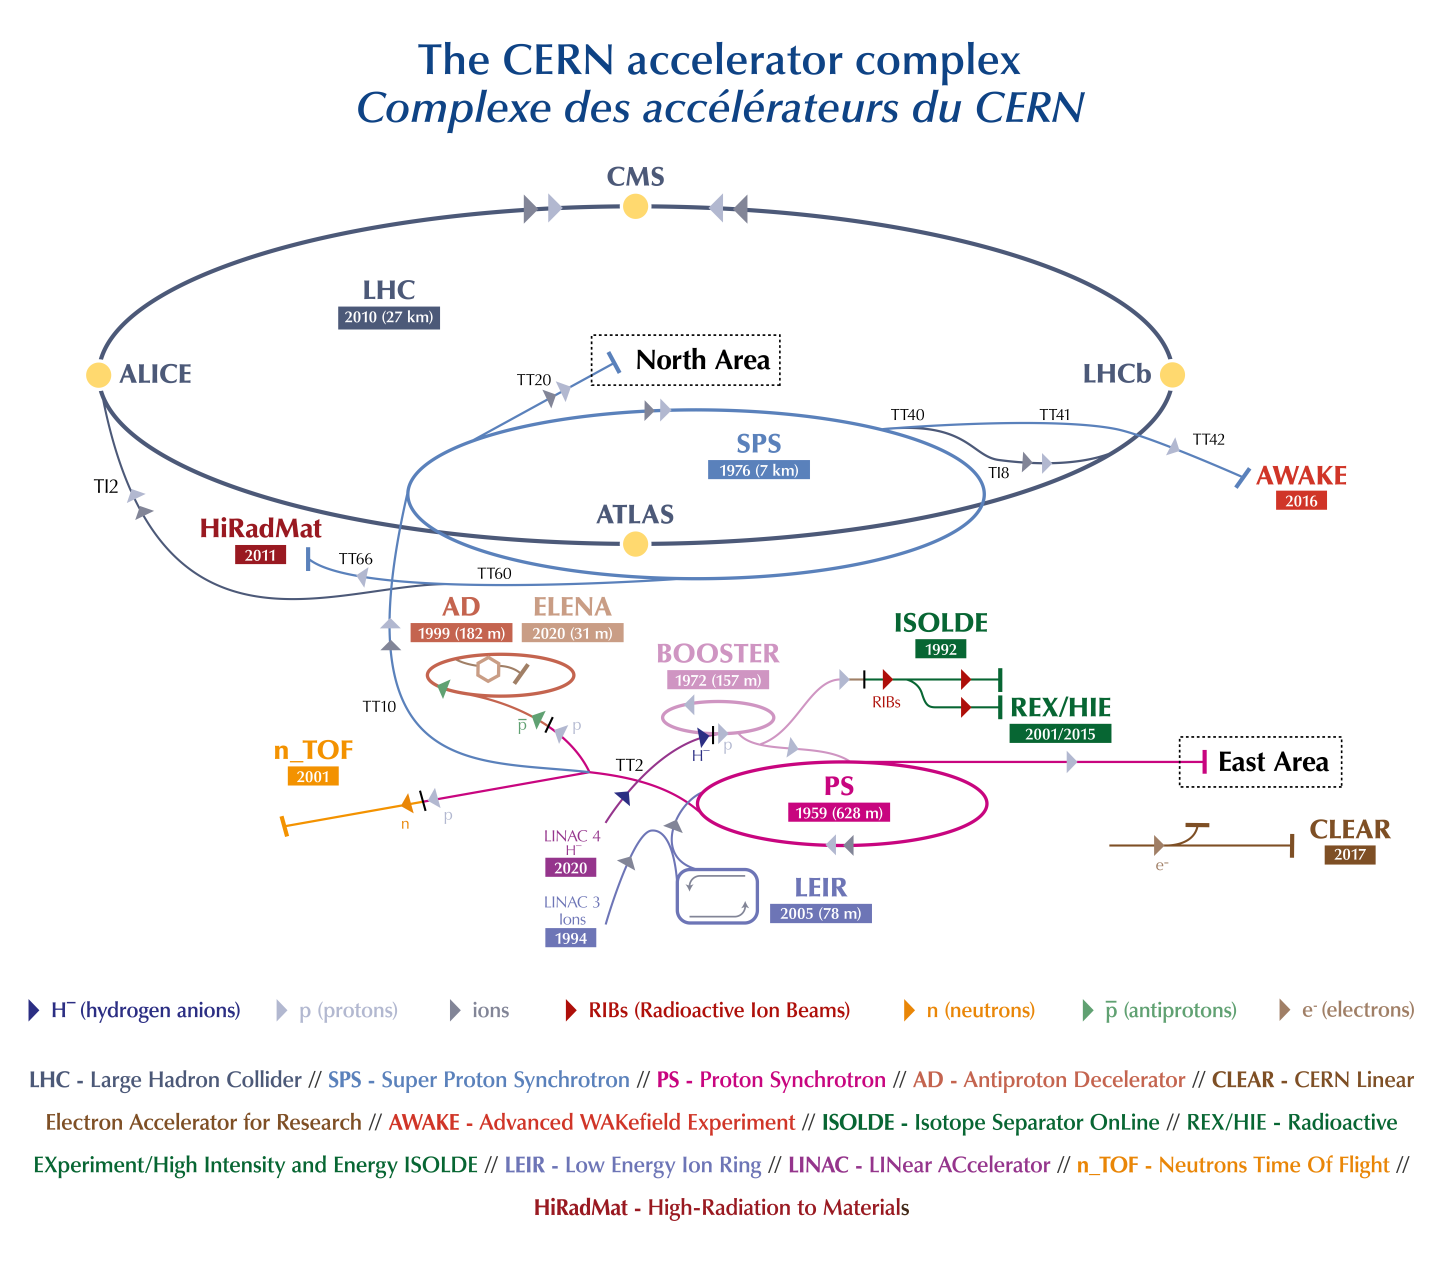
\includegraphics[width=0.9\textwidth]{LHC.png}
  \caption{Le complexe d'accélérateurs du CERN.}
  \label{fig:lhc_complex}
\end{center}
\end{figure}

\subsection{Les expériences}

Le LHC étant un collisionneur circulaire, il est possible de faire se croiser les faisceaux de protons à plusieurs endroits. Plusieurs dispositifs expérimentaux sont installés, aux points de croisements. Le LHC est divisé en huit sections (ou points) et compte quatre croisements avec quatre expériences majeures : ALICE \cite{alice}, ATLAS \cite{atlas}, CMS \cite{cms} et LHCb \cite{lhcb}.

\begin{description}
  \item[A Large Ion Collider Experiment (ALICE)] Au point 2, cette expérience est principalement dédiée à l'étude du déconfinement de la matière nucléaire, le plasma de quarks et gluons. Les données qu'elle utilise sont celles issues des collisions d'ions lourds (Pb-Pb ou \Pproton{}-Pb), mais les collisions \Pproton{}-\Pproton{} sont aussi utilisées afin de calibrer le détecteur.
  \item[A Toroidal LHC ApparatuS (ATLAS) / Compact Muon Solenoid (CMS)]
  \begin{sloppypar}
   Respectivement aux points 1 et 5, ce sont les deux expériences généralistes du LHC. En effet, le programme de physique de ATLAS et CMS est très vaste, et couvre la recherche du boson de Higgs et de nouvelle physique, les mesures de précisions du Modèle Standard, ainsi que la recherche de candidats matière noire. Souvent mises en concurrence, ces expériences sont pourtant complémentaires. Ainsi, on a pu voir le 4 juillet 2012 ces deux expériences annoncer conjointement la découverte d'une particule compatible avec le boson de Higgs \cite{higgs_atlas,higgs_cms}, chacune confirmant ainsi les résultats de l'autre.
  \end{sloppypar}
  \item[Large Hadron Collider beauty (LHCb)] Au point 8, c'est la dernière expérience majeure du LHC, principalement dédiée aux mesures de précision du Modèle Standard ainsi qu'à l'étude de la violation de la symétrie CP, grâce à l'étude poussée du quark $b$. La collaboration LHCb a d'ailleurs annoncé récemment avoir observé pour la première fois la violation de symétrie CP dans le système $B_s$ \cite{lhcb_bs}, telle que prévue par le Modèle Standard. Cette récente découverte permet de contraindre encore plus fortement certains modèles de nouvelle physique.
\end{description}

Il existe 3 autres expériences au LHC, installées à proximité des points de croisement des faisceaux : LHCf \cite{lhcf}, MoEDAL \cite{moedal} et TOTEM \cite{totem}.

\begin{description}
  \item[Large Hadron Collider forward (LHCf)] Situé à environ $140\,\mathrm{m}$ de part et d'autre d'ATLAS, ce détecteur étudie les particules créées à très petits angles, principalement afin de simuler la production de rayons cosmiques de très haute intensité en laboratoire.
  \item[Monopole and Exotics Detector at the LHC (MoEDAL)] 
    \begin{sloppypar}
  Située juste en aval de LHCb, MOeDAL traque les monopôles magnétiques, grâce à un détecteur spécialement conçu pour ce rôle.
    \end{sloppypar}
  \item[TOTal Elastic and diffractive cross section Measurement (TOTEM)] Destinée à mesurer la section efficace élastique des collisions \Pproton{}-\Pproton{}, cette expérience, située dans la même caverne que CMS, étudie les particules créées à très petits angles. Elle peut également faire des mesures précises de la luminosité du LHC.
\end{description}


\subsection{Luminosité}

La luminosité instantanée est une variable clé dans un accélérateur de particules. Exprimée en unités \si{\per\square\cm\per\second} (ou plus régulièrement \si{\hertz\per\micro\barn}), elle représente le taux de collisions au point d'interaction. Elle est exprimée au LHC en fonction de diverses variables caractéristiques telles que la forme des paquets de protons, leur énergie,... etc.

La luminosité instantanée est la luminosité évaluée pendant une période infinitésimale donnée. Elle vaut :
\begin{equation}
 \mathcal{L}_\textrm{inst} = \frac{\gamma f n_p N_P^2}{4 \pi \epsilon_n \beta^{*}} = \frac{f n_p N_P^2}{4 \pi \sigma_x \sigma_y }
\end{equation} 
où $\gamma$ est le boost de Lorentz, $f$ est la fréquence de rotation des paquets, $n_p$ est le nombre de paquets de protons circulant dans le LHC, $N_p$ est le nombre de protons par paquet, $\epsilon_n$ est l'émittance transversale (mesure du parallélisme du faisceau). Pour favoriser les collisions, les deux faisceaux sont resserrés à l'approche du point de collision. $\beta^*$ mesure la distance entre le point d'interaction et le point où le faisceau double de largeur. Les $\sigma_{x,y}$ sont les tailles transversales du faisceau au point d'interaction. Les valeurs des différents paramètres du faisceau sont indiquées dans le tableau \tablename{\ref{tab:lhc_beam}} pour divers scenarii.

\begin{table} [H]
\begin{center}
  \begin{tabular}{cc} 
  \noalign{\smallskip}\hline\noalign{\smallskip}
  Caractéristiques & LHC Run II \\ 
  \noalign{\smallskip}
  \hline \hline
  \noalign{\smallskip}
  Énergie par proton (\si{\TeV}) & \num{6.5} \\
  $\mathcal{L}$ ( \si{\femto \barn^{-1}}) & \num{163.5} (\figurename{\ref{fig:cms_lumi}})  \\ 
  $f$ (\si{\hertz}) & \num{11246} \\
  \noalign{\smallskip}\hline\noalign{\smallskip}
  Intervalle entre croisements de paquet (\si{\nano\second}) & \num{25}\\
  Nombre de paquets & \num{2808} \\
  Protons par paquet (\num{e11}) & \num{1.2}\\
  $\beta^*$ (\si{\meter}) & \num{0.55} \\ 
  \noalign{\smallskip}\hline\noalign{\smallskip}
  \end{tabular}
  \caption{Les différents paramètres du faisceau  \Pproton{}-\Pproton{} du LHC \cite{CMStechnical}.}
  \label{tab:lhc_beam}
\end{center}
\end{table}

A partir de la luminosité instantanée, on peut déduire le nombre d'évènements observés $N$, d'un processus étudié $i$, par l'équation:
\begin{equation}
N_i = \int \mathcal{L}_\mathrm{inst} \sigma_i dt
\end{equation}
avec  $\sigma_i$ la section efficace du processus $i$.

\begin{figure}
\begin{center}
  \subcaptionbox{\label{fig:cms_lumi}}[0.48\textwidth]{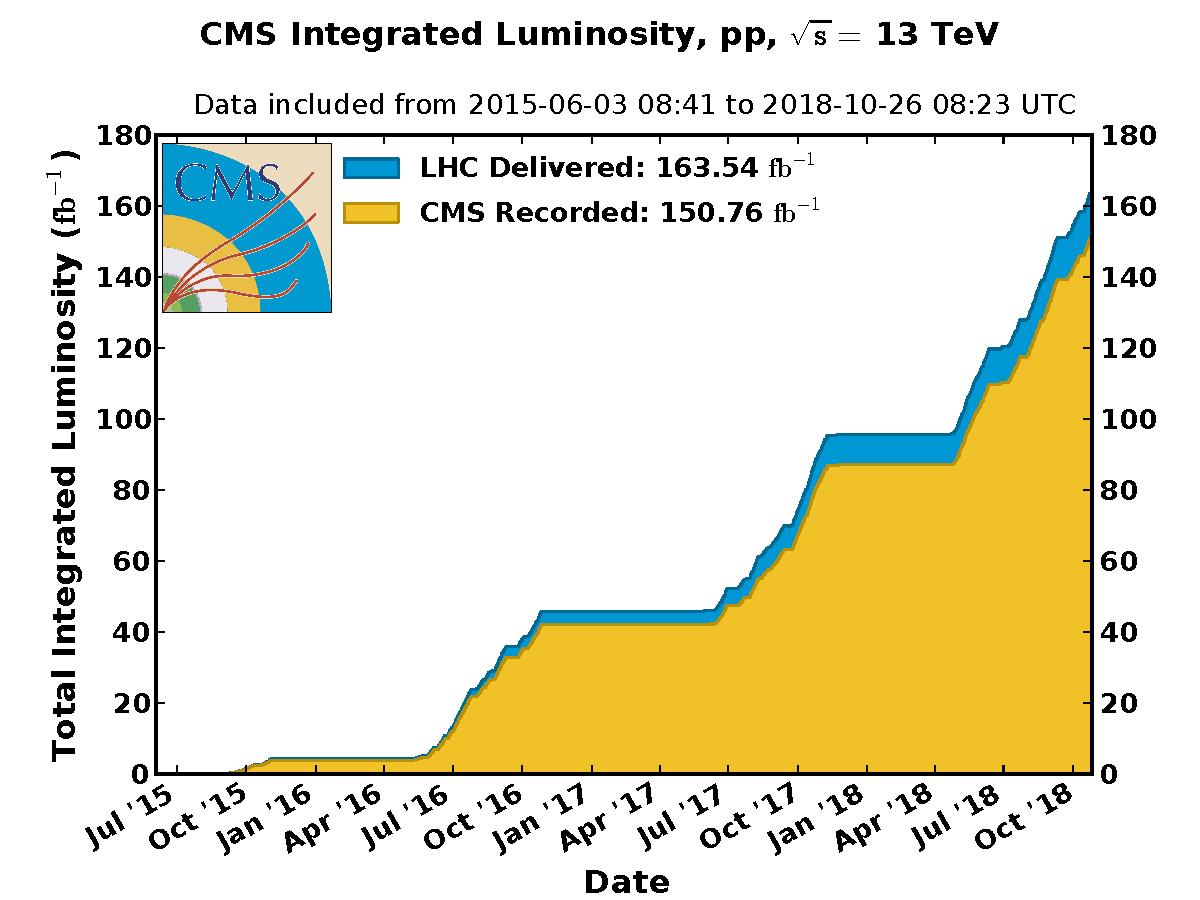
\includegraphics[width=0.48\textwidth]{LumiRun2.pdf}}
  \subcaptionbox{\label{fig:cms_pu}}[0.48\textwidth]{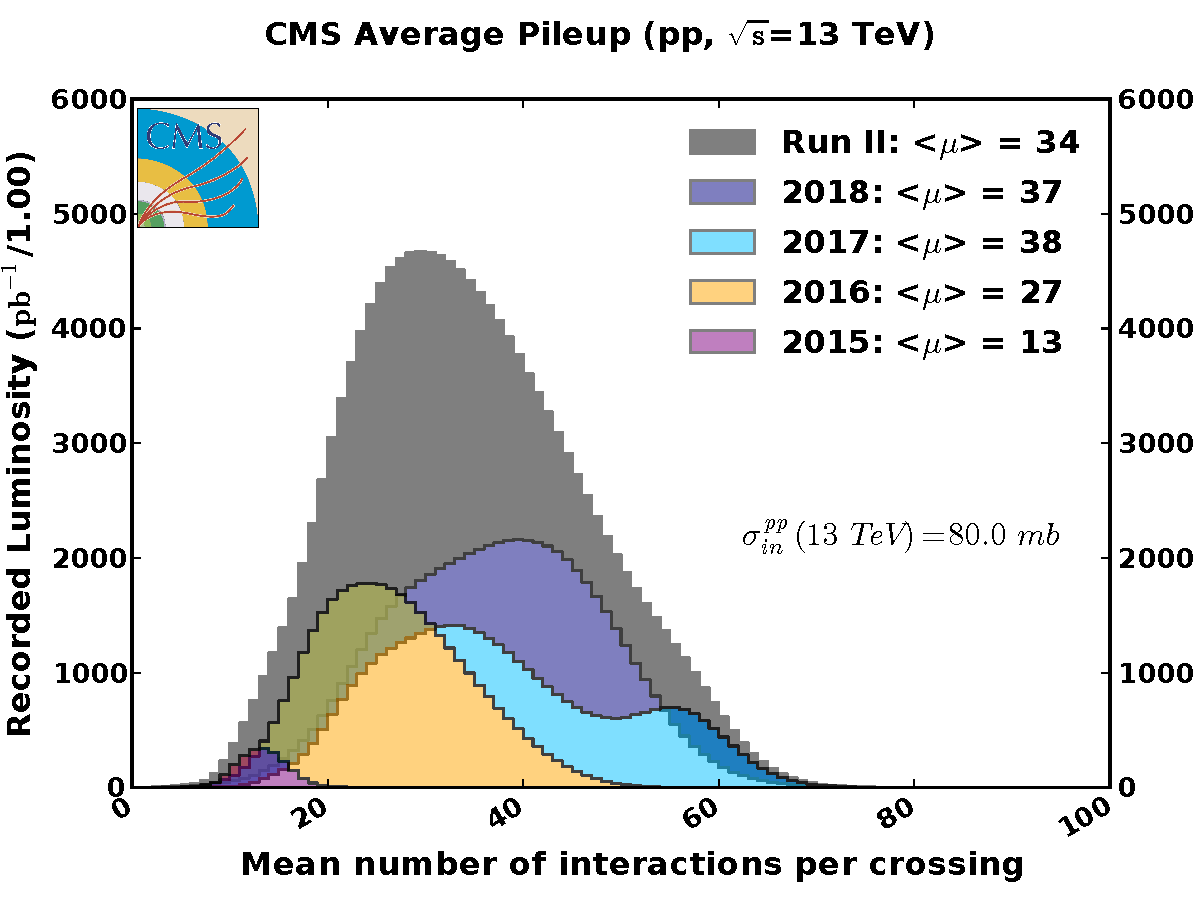
\includegraphics[width=0.48\textwidth]{PURun2.pdf}}
  \caption{(\subref{fig:cms_lumi}) Luminosité intégrée collectée par l'expérience CMS au cours du Run II du LHC. (\subref{fig:cms_pu}) Nombre moyen d'interactions par croisement de faisceaux observées pendant la prise de données de différentes années du Run II.}
  \label{fig:lumi}
\end{center}
\end{figure}

\subsection{Empilement}

Les protons se déplaçant par paquets, plusieurs interactions \Pproton{}-\Pproton{} peuvent se produire lors d'un même croisement de  faisceaux. La collision principale, centre d'intérêt des analyses, est nommée "évènement dur". Les autres collisions (élastiques ou inélastiques) parasitent l'événement dur. Cet effet est communément appelé empilement (\emph{pile-up} (PU) en anglais). Pour le Run-II, le nombre moyen d'interactions par croisement $\langle \mu \rangle$ est d'environ $34$.

\begin{description}
\item[empilement synchrone] 
  \begin{sloppypar}
Il est produit en même temps que l'évènement dur. A chaque collision correspond un vertex, qui est le lieu de rencontre de deux protons. Le vertex principal (dur) est celui pour lequel la somme quadratique des impulsions transverses ($\pt$) des particules chargées reconstruites dans le détecteur est la plus grande. Les autres sont considérés comme vertex d'empilement. Les particules provenant de vertex d'empilement laissent dans le détecteur des bruits parasites.
  \end{sloppypar}
\item[empilement asynchrone] Il est principalement causé par le temps de réponse des détecteurs. Cet empilement est d\^u au recouvrement entre des évènements en cours de traitement, les suivants et les précédents.
\end{description}

L'empilement se traduit directement par une augmentation du nombre de vertex d'interactions reconstruits par le détecteur. On présente sur la figure \figurename{\ref{fig:cms_pu}} le nombre d'interactions moyen par croisement de faisceau, pour différentes années. En absence  d'empilement, une seule interaction serait enregistrée.


\section{L'expérience CMS (\emph{Compact Muon Solenoid})}

Le \emph{compact muon solenoid} est une expérience du LHC installée sur le territoire français près de Cessy dans l'Ain. Les motivations étant diverses, de l'étude de la brisure de symétrie électrofaible à la recherche de nouvelle physique (supersymétrie, matière noire, ...), on qualifie cette expérience de généraliste. 

\begin{figure}
\begin{center}
  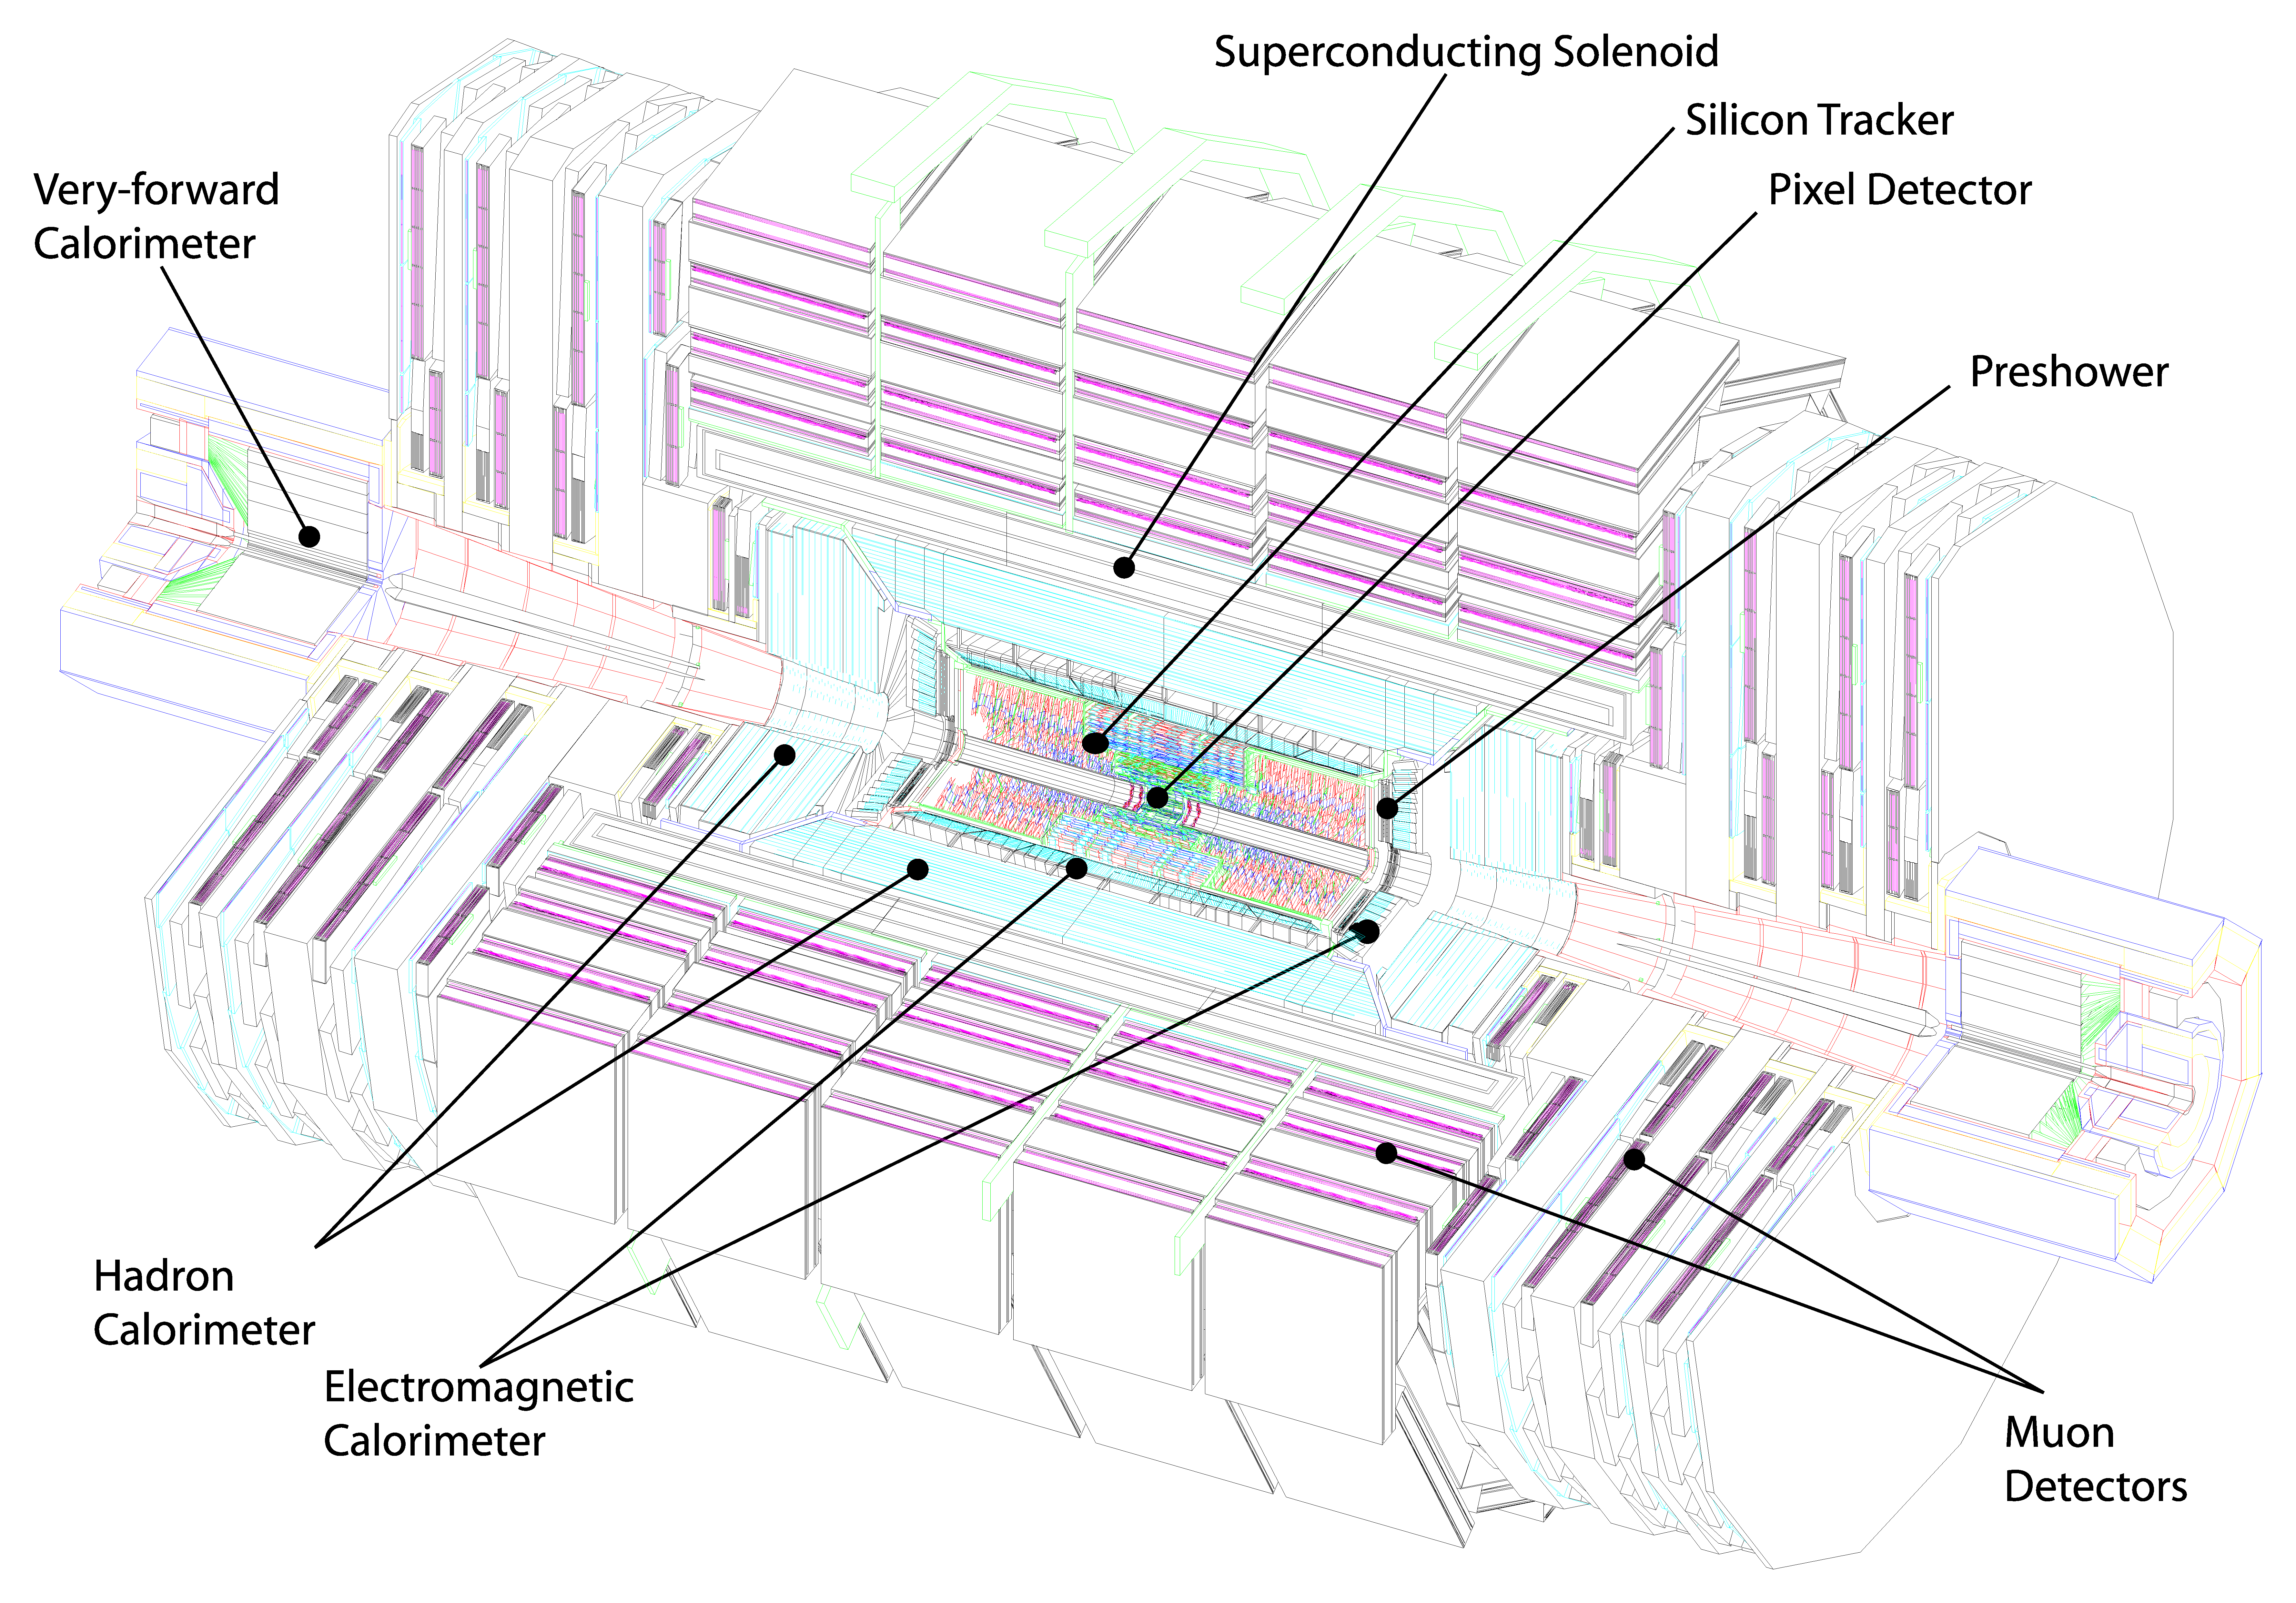
\includegraphics[width=0.7\textwidth]{CMS_2.pdf}
  \caption{Vue en perspective du détecteur CMS et de ses sous-détecteurs \cite{CMStechnical}.}
  \label{fig:cms}
\end{center}
\end{figure}

Une vue éclatée du détecteur CMS est représentée sur la figure \figurename{\ref{fig:cms}}. Ce détecteur est composé de plusieurs sous-parties possédant chacune une spécialité de détection pour différents éléments (électrons, muons, jets, ...).% Des schémas fonctionnels présentant les zones de mesure d'une désintégration du quark top dans CMS sont présentés à la figure \figurename{\ref{fig:cms_event}}.

%\begin{figure}
%\begin{center}
%  \subcaptionbox{\label{fig:cms_event1}}[0.48\textwidth]{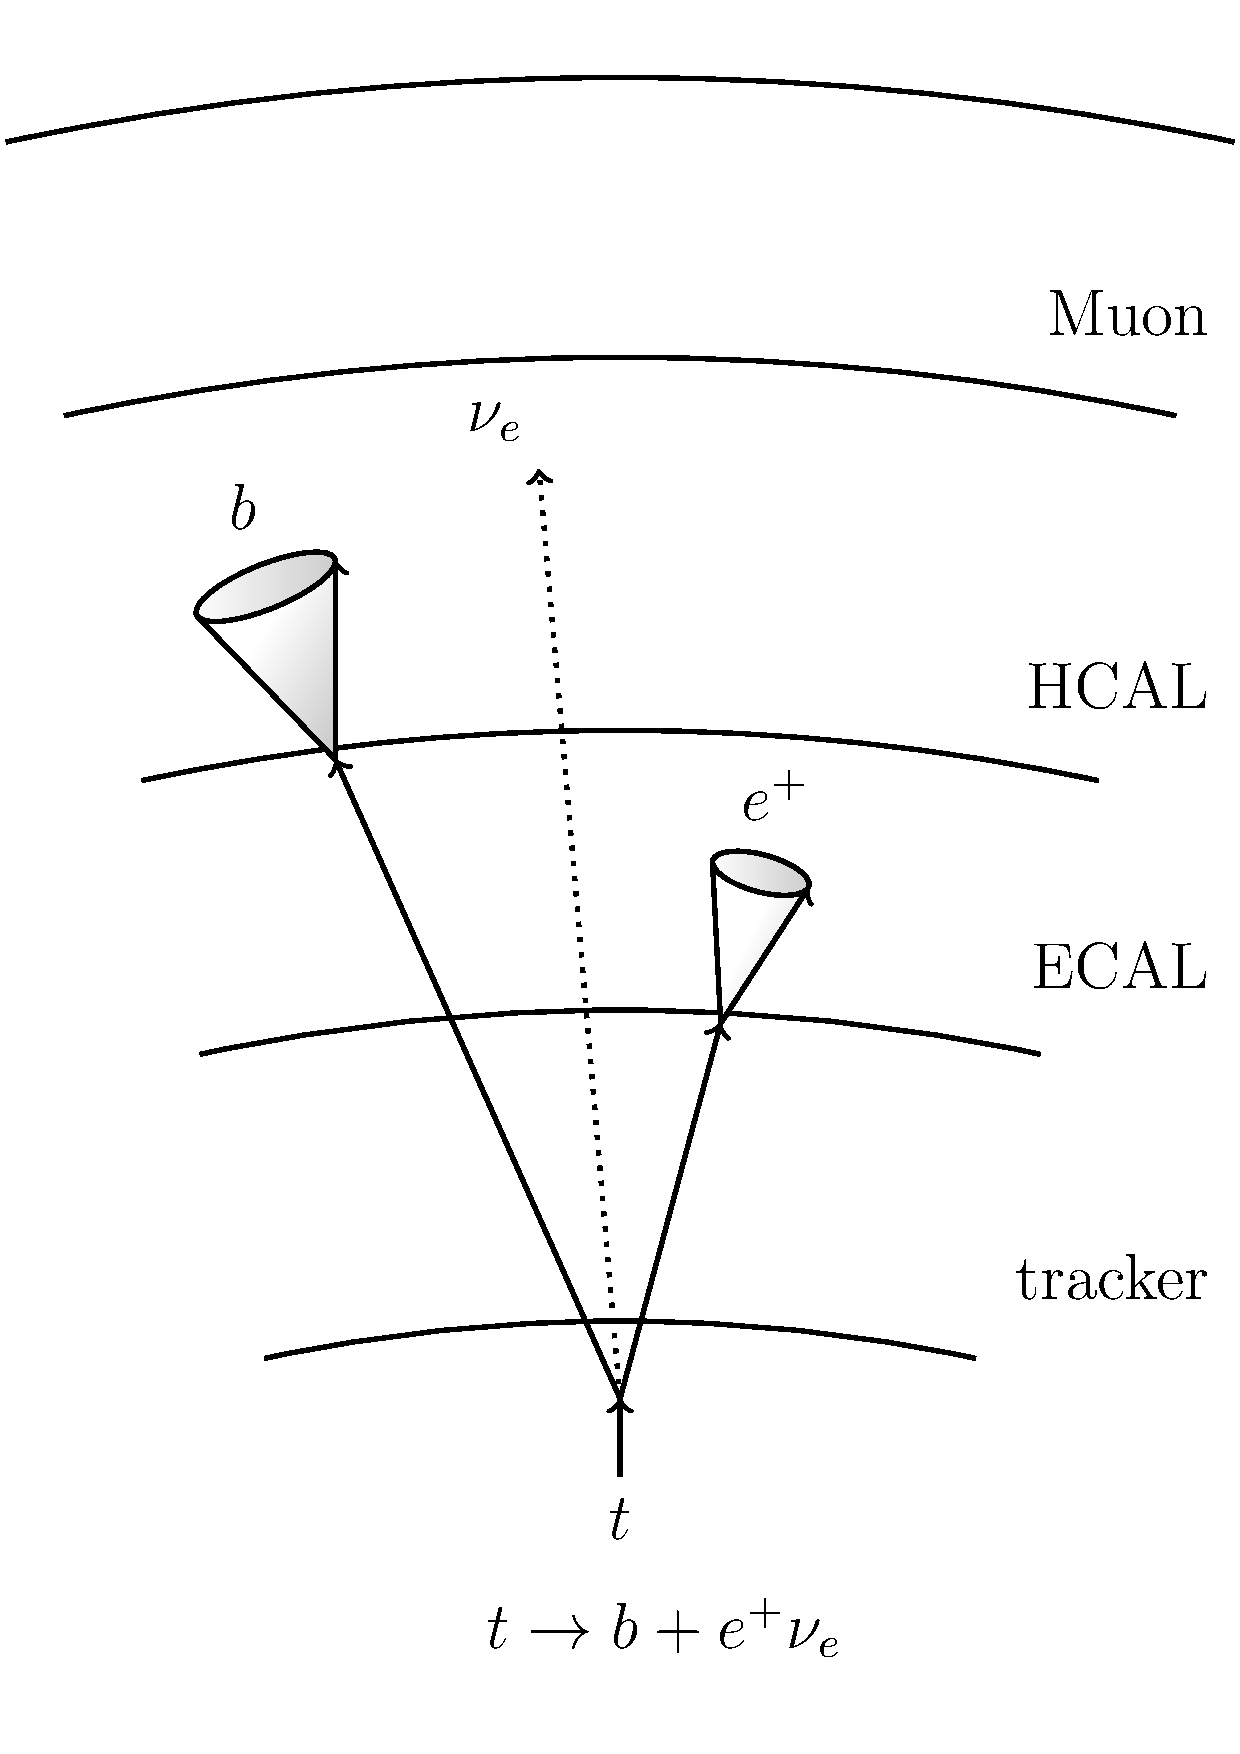
\includegraphics[width=0.3\textwidth]{cms_top1.pdf}}
%  \subcaptionbox{\label{fig:cms_event2}}[0.48\textwidth]{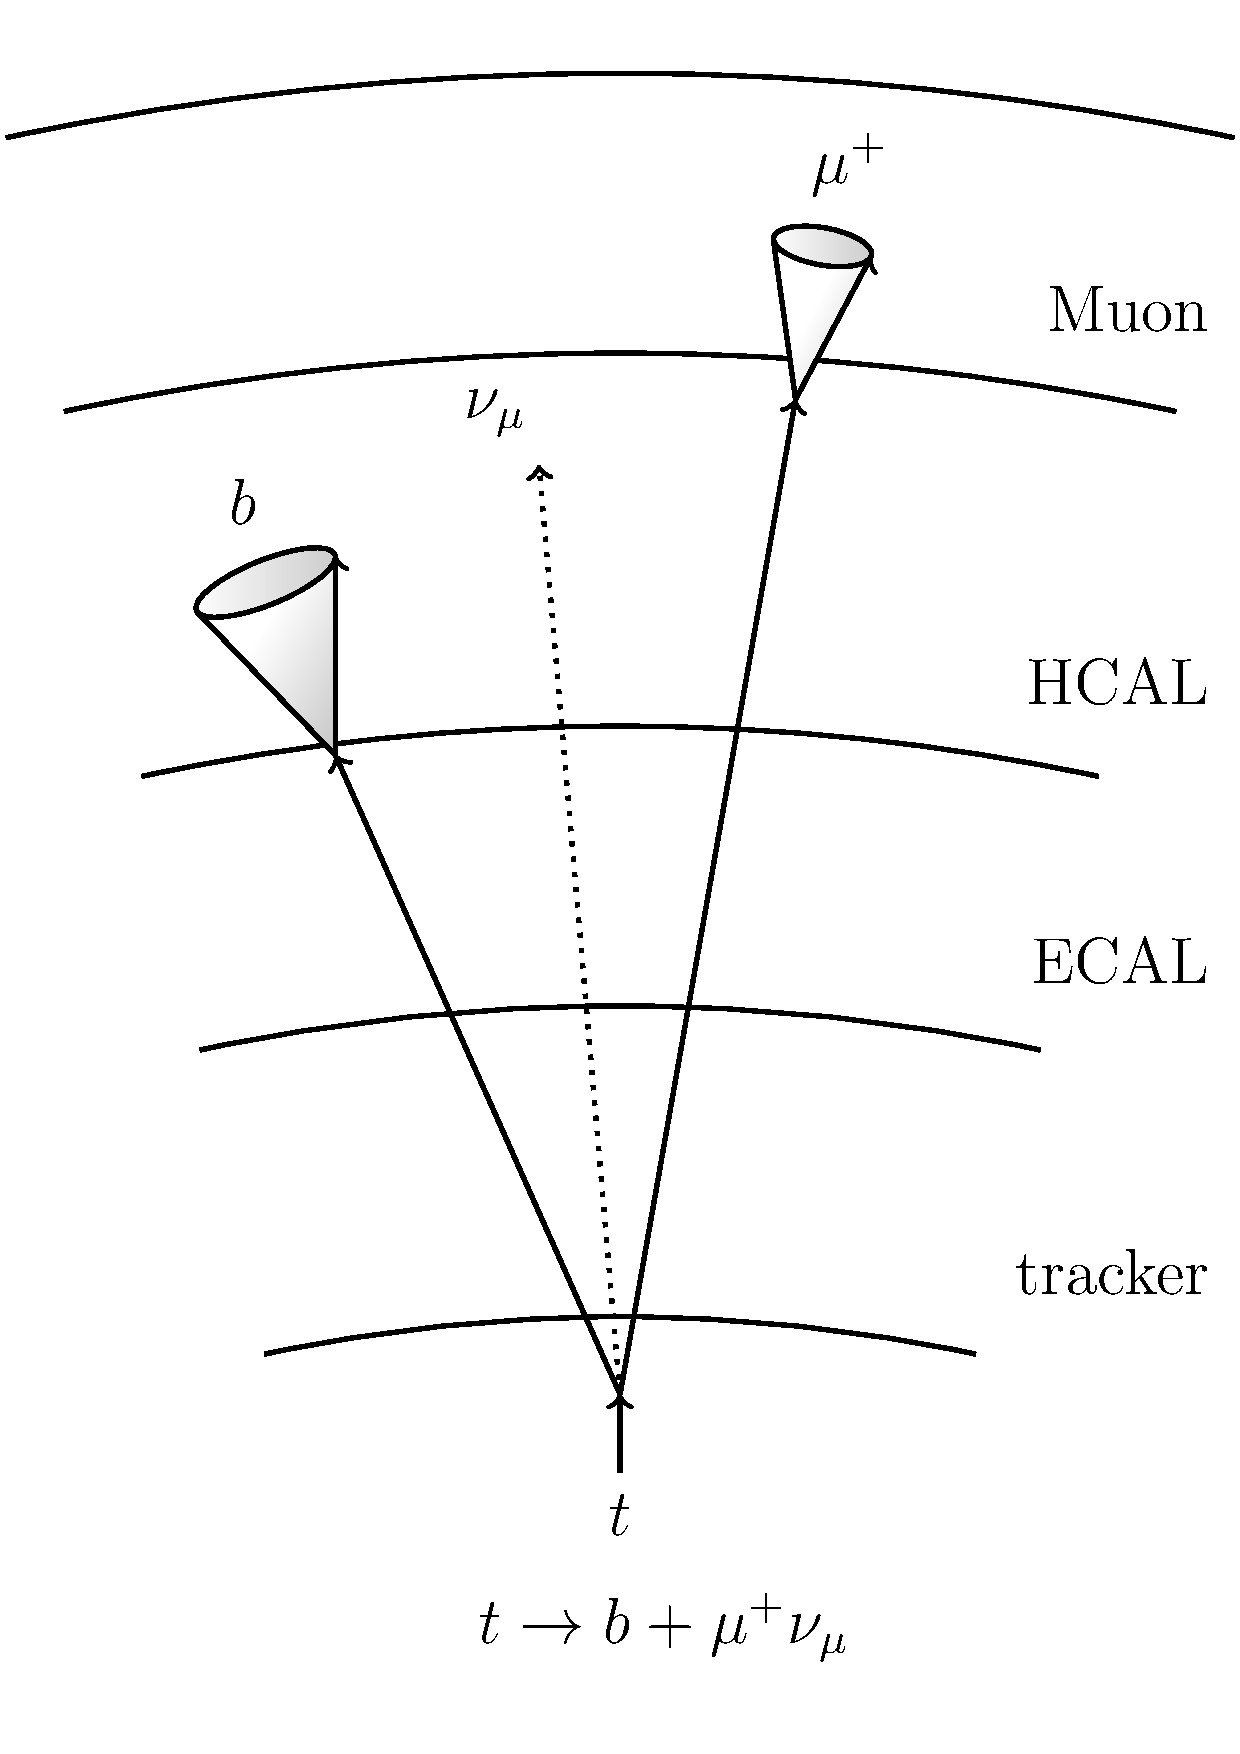
\includegraphics[width=0.3\textwidth]{cms_top2.pdf}}
%  \caption{(\subref{fig:cms_event1}) Schéma d'un évènement de désintégration électronique du quark top dans le détecteur CMS. (\subref{fig:cms_event2}) Schéma d'un évènement de désintégration muonique du quark top dans le détecteur CMS.}
%  \label{fig:cms_event}
%\end{center}
%\end{figure}
%

\subsection{Système de coordonnées}\label{chap3:CMS}

  CMS (figure \figurename{\ref{fig:cms}}) est situé au point 5 du LHC. Il s'agit d'un détecteur 
   compact, cylindrique mesurant \SI{28.7}{\m} de long avec un rayon de \SI{7.5}{\m}, pour un poids de \SI{14000}{\tonne}. Il est composé de plusieurs sous-détecteurs, organisés en couches successives de détections. Pour décrire plus en détails ces sous-détecteurs, il est nécessaire de définir un système de référence, où l'origine est donnée par le centre du détecteur. L'axe $x$ pointe vers le centre de l'anneau du LHC, et l'axe $z$ est tangent à la direction du faisceau. L'axe $y$, perpendiculaire aux deux autres axes, pointe vers le haut (voir figure \figurename{\ref{fig:coord}}). 

    \begin{figure}
       	\begin{center}
            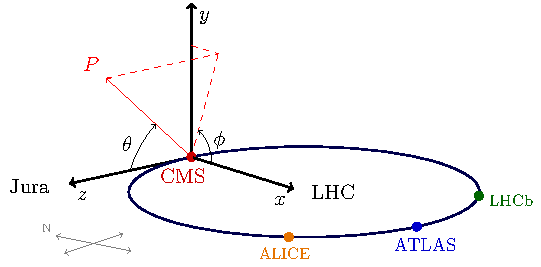
\includegraphics[scale=1]{cms_coordinate_system.pdf}
       	\end{center}
           \caption{Système de coordonnées du détecteur CMS par rapport à l'anneau du LHC \cite{CMStechnical}.}
           \label{fig:coord}
    \end{figure}
    
L'angle azimutal $\phi \in \left[-\pi, \pi\right]$ est mesuré dans le plan $(x,y)$, à partir de l'axe $x$. L'angle $\theta$, lui, est défini à partir de l'axe $z$ dans le plan transverse $(y,z)$. Il est plus commode d'utiliser la pseudo-rapidité $\eta$ plutôt que $\theta$, puisque la densité de production de particules est constante suivant $\eta$, mais pas suivant $\theta$. De plus, pour des particules ultra-relativiste la pseudo-rapidité tend vers la rapidité qui est une quantité additive. On définit la pseudo-rapidité par
\begin{equation}
  \eta = -\ln\left[\tan\left(\frac{\theta}{2}\right)\right] = \frac{1}{2} \ln\left(\frac{\abs{\vec{p}} + p_z}{\abs{\vec{p}} - p_z}\right)  
\end{equation}
  où $p_z$ est la projection de l'impulsion le long de l'axe du faisceau.
  
  Du fait de la structure interne des protons, lors d'une collision, l'impulsion totale selon l'axe du faisceau est inconnue. De plus, le détecteur n'est pas hermétique et certaines particules (dont les neutrinos) échappent à la détection ce qui implique que l'on ne peut pas déduire par reconstruction, non plus, l'impulsion $p_z$.  Pour contrer ce problème, la stratégie est d'utiliser le fait que la somme vectorielle des impulsions sera nulle dans le plan transverse. Ainsi on introduit des variables relatives à ce plan transverse $(x,y)$ : l'impulsion transverse $\pt$ et l'énergie transverse $\ET$. On a ainsi
\begin{align*}
  \pt &= \sqrt{p_x^2 + p_y^2} = \frac{\abs{\vec{p}}}{\cosh\eta} \\
  \et &= E \sin\theta = \frac{E}{\cosh\eta}
\end{align*}
Également, on peut définir la distance angulaire $\Delta R$ entre deux particules $i$ et $j$ telle que:
\begin{equation}
    \Delta R_{ij} = \sqrt{(\eta_i -\eta_j)^2 + (\phi_i -\phi_j)^2 } = \sqrt{\Delta\eta^2(i,j) + \Delta\phi^2(i,j)}
\end{equation}
Cette dernière quantité est très utile pour l'estimation de l'isolation d'une particule.

\subsection{Aimant solénoïdal}
Le solénoïde supraconducteur est un élément central de CMS. Il fournit un champ magnétique de \SI{3.8}{\tesla}. De forme cylindrique de rayon \SI{6}{\m}, long de \SI{12.5}{\meter}, il est parcouru par un courant électrique de \SI{19.14}{\kilo\ampere}. Afin de maintenir son état supraconducteur, l'aimant est refroidi par un système de cryostats fonctionnant à l'hélium superfluide. Il est ainsi constamment maintenu à une température de \SI{1.9}{\kelvin}.

On a déjà vu précédemment l'intérêt d'un puissant champ magnétique. En effet, la trajectoire d'une particule chargée se courbe en présence d'un champ magnétique, avec un rayon de courbure proportionnel à son impulsion :
\begin{align*}
  r &= \frac{\| \vec{p} \|}{qB}
\end{align*}
avec $r$ le rayon de courbure de la trajectoire, $p$ l'impulsion, $q$ la charge de la particule et $B$ l'intensité du champ magnétique. Plus $r$ est petit, plus mesurer la courbure de la trajectoire d'une particule est aisée, puisque la courbure de la trajectoire est plus prononcée. Afin d’assurer de bonnes performances sur l’identification des particules, il est nécessaire d'utiliser un champ magnétique puissant pour minimiser $r$.

\subsection{Le trajectographe : pixels et pistes de silicium}

Le trajectographe est l'un des composants les plus importants de CMS. En plus de la reconstruction des vertex d'interactions, il est chargé de reconstruire la trajectoire courbée des particules chargées, et ainsi d'en déduire leur impulsion. Il s'agit d'un cylindre d'une longueur de \SI{5.5}{\m} et de \SI{1.1}{\m} de rayon. Le trajectographe, conçu pour couvrir une région angulaire entre $0 < \aeta < \num{2.5}$, est composé de deux sous-parties.

Le détecteur à pixels est la partie la plus interne du trajectographe, il est composé de quatre couches de détection \cite{CMStrackerUpdate} situées au plus proche du point de collision (à $r = \SI{2.9}{\cm}$, $r = \SI{6.8}{\cm}$, $r = \SI{10.9}{\cm}$ et $r = \SI{16}{cm}$), et de trois disques (bouchons) disposés à chaque extrémité. Dans ce détecteur à silicium, on dénombre \num{66e6} pixels, mesurant chacun \num{100}$\times$\SI{150}{\square\um}, pour une superficie totale de détection d'environ \SI{1}{\square\m}. 
La résolution en \pt, obtenue à partir des algorithmes de reconstructions des traces du trajectographe, est présentée sur la figure \figurename{\ref{fig:pixel_resolution}}. On peut voir une résolution d'environ \SI{1}{\%} dans le tonneau et  d'environ \SI{2}{\%} dans les bouchons.
\newline 

Le detecteur à micropistes, englobant le détecteur à pixels, est composé de 10 couches en silicium. Cela représente environ 10 millions de micropistes. Quatre sous-ensembles sont dénombrables : 

\begin{description}
  \item[Le TIB] (\emph{Tracker Inner Barrel}) Composée de quatre couches de micropistes, c'est la partie interne du tonneau du trajectographe.
  \item[Le TID] (\emph{Tracker Inner enDcaps}) Avec trois couches de détection, cette partie constitue les bouchons internes, et complète le TIB.
  \item[Le TOB] (\emph{Tracker Outer Barrel}) Cette partie externe est constituée de six couches de micropistes. Elle entoure le TIB.
  \item[Le TEC] (\emph{Tracker EndCaps}) Composée de neuf couches, elle forme les deux bouchons externes et complète le TOB.
\end{description}

\begin{figure} 
\begin{center}
    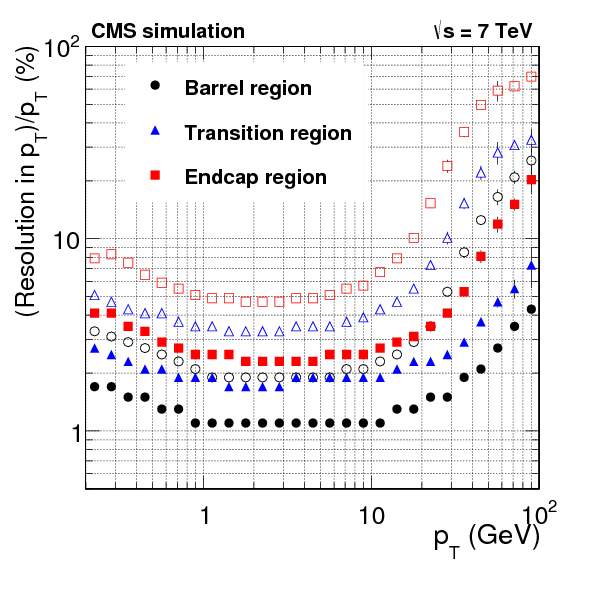
\includegraphics[width=0.5\textwidth]{ptresolution.png}
    \caption{Résolution en impulsion transverse des traces reconstruites \cite{Collaboration_2014}.}
    \label{fig:pixel_resolution}
\end{center}
\end{figure}

L'agencement du trajectographe, avec les détecteurs à pixels et à micropistes, est présenté en détail figure \figurename{\ref{fig:tracker}}.

\begin{figure}
\begin{center}
  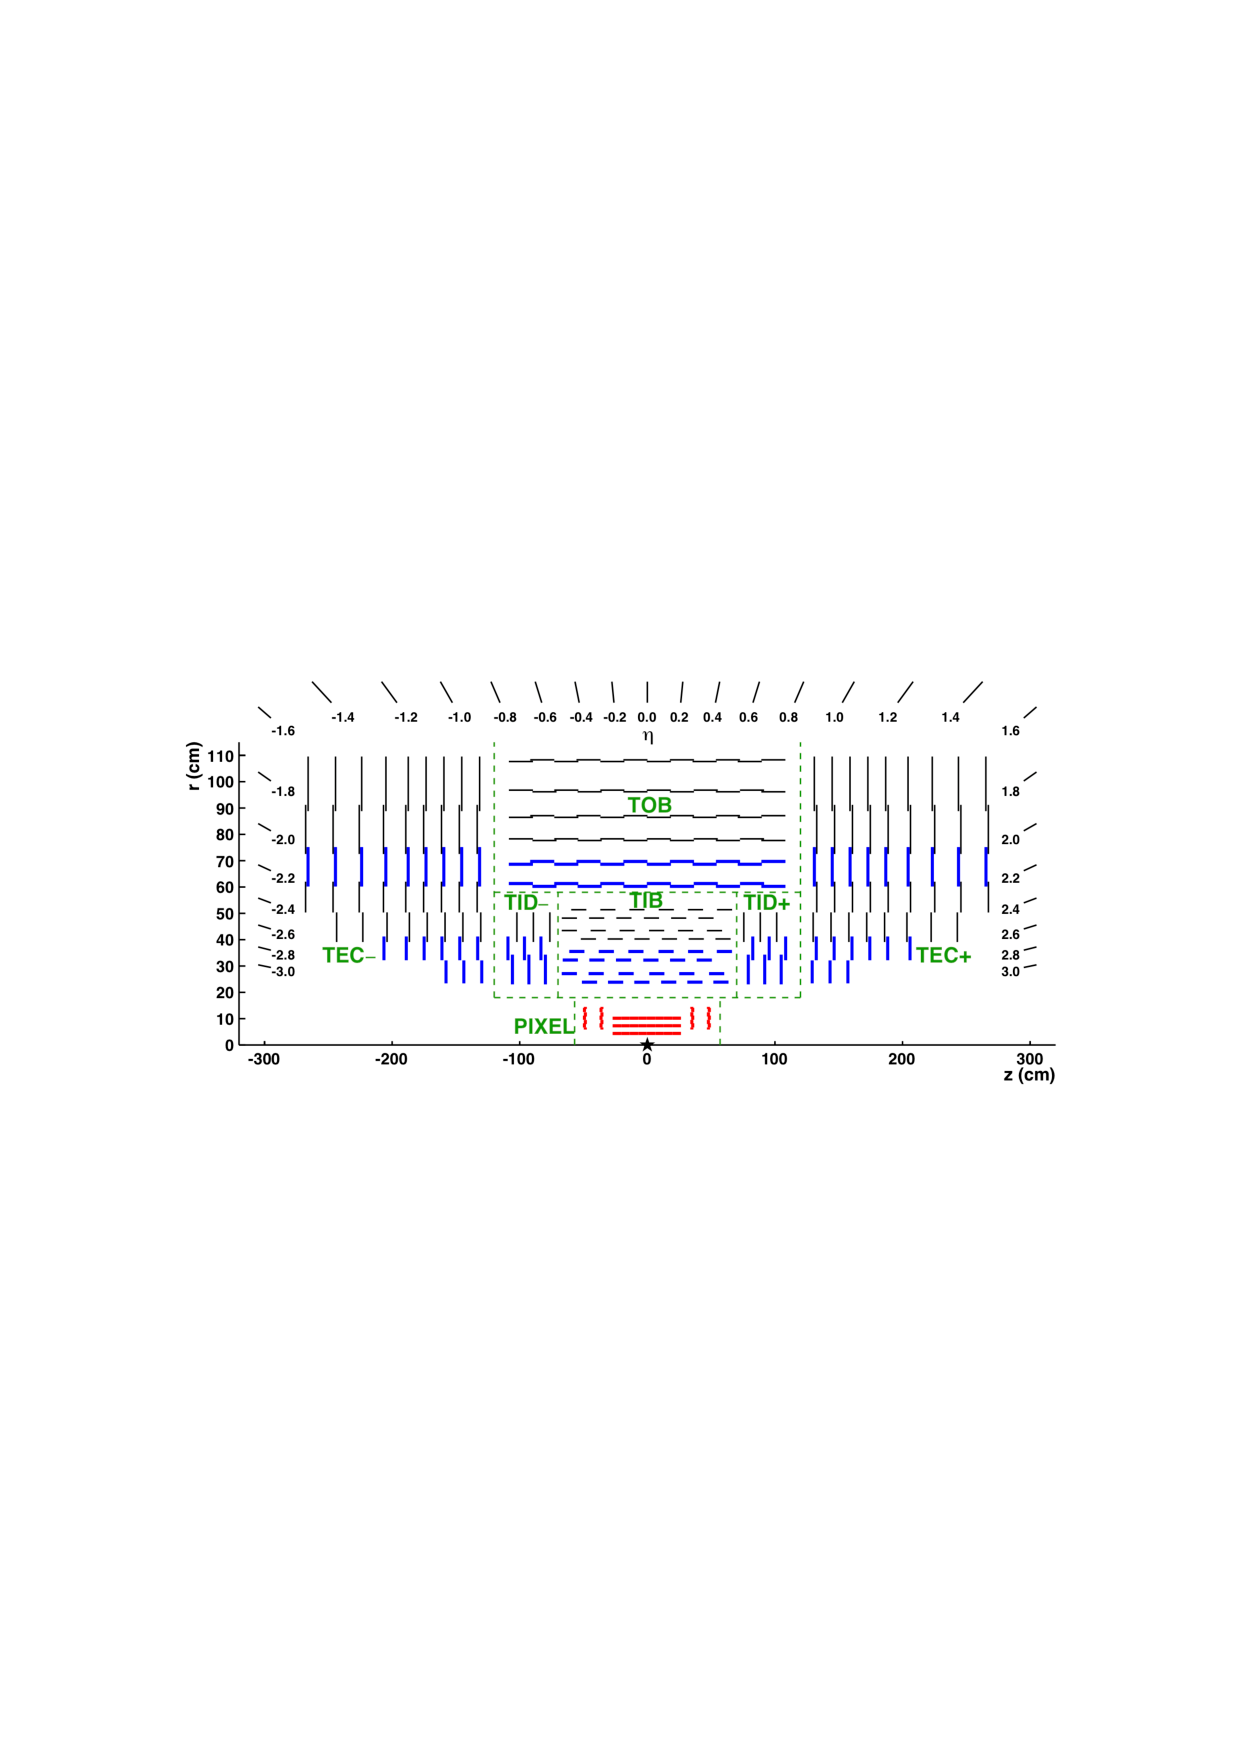
\includegraphics[width=0.8\textwidth]{tracker2.pdf}
  \caption{Vue détaillée du trajectographe de l'expérience CMS \cite{CMStechnical}.}
  \label{fig:tracker}
\end{center}
\end{figure}




\subsection{Calorimètre électromagnétique}


Enrobant le trajectographe, le calorimètre électromagnétique (ECAL) capte et mesure l'énergie des électrons et des photons. Il s'agit d'un détecteur à scintillations formé de cristaux de tungstate de plomb ($PbWO_4$). Comme le trajectographe il est composé de deux parties : le tonneau (EB, pour \emph{ECAL Barrel}) couvrant la région angulaire $0 < \abs{\eta} < \num{1.479}$, avec 61200 cristaux ; et le bouchon (EE, pour \emph{ECAL Endcap}) couvrant la région angulaire $\num{1.479} < \abs{\eta} < 3$, avec  15000 cristaux au total. La figure \figurename{\ref{fig:ecaltrans}} présente une vue schématique de la structure du ECAL. Il est à noter que le ECAL est impliqué également dans le déclenchement (voir section \ref{declenchement}).


\begin{figure}
\begin{center}
  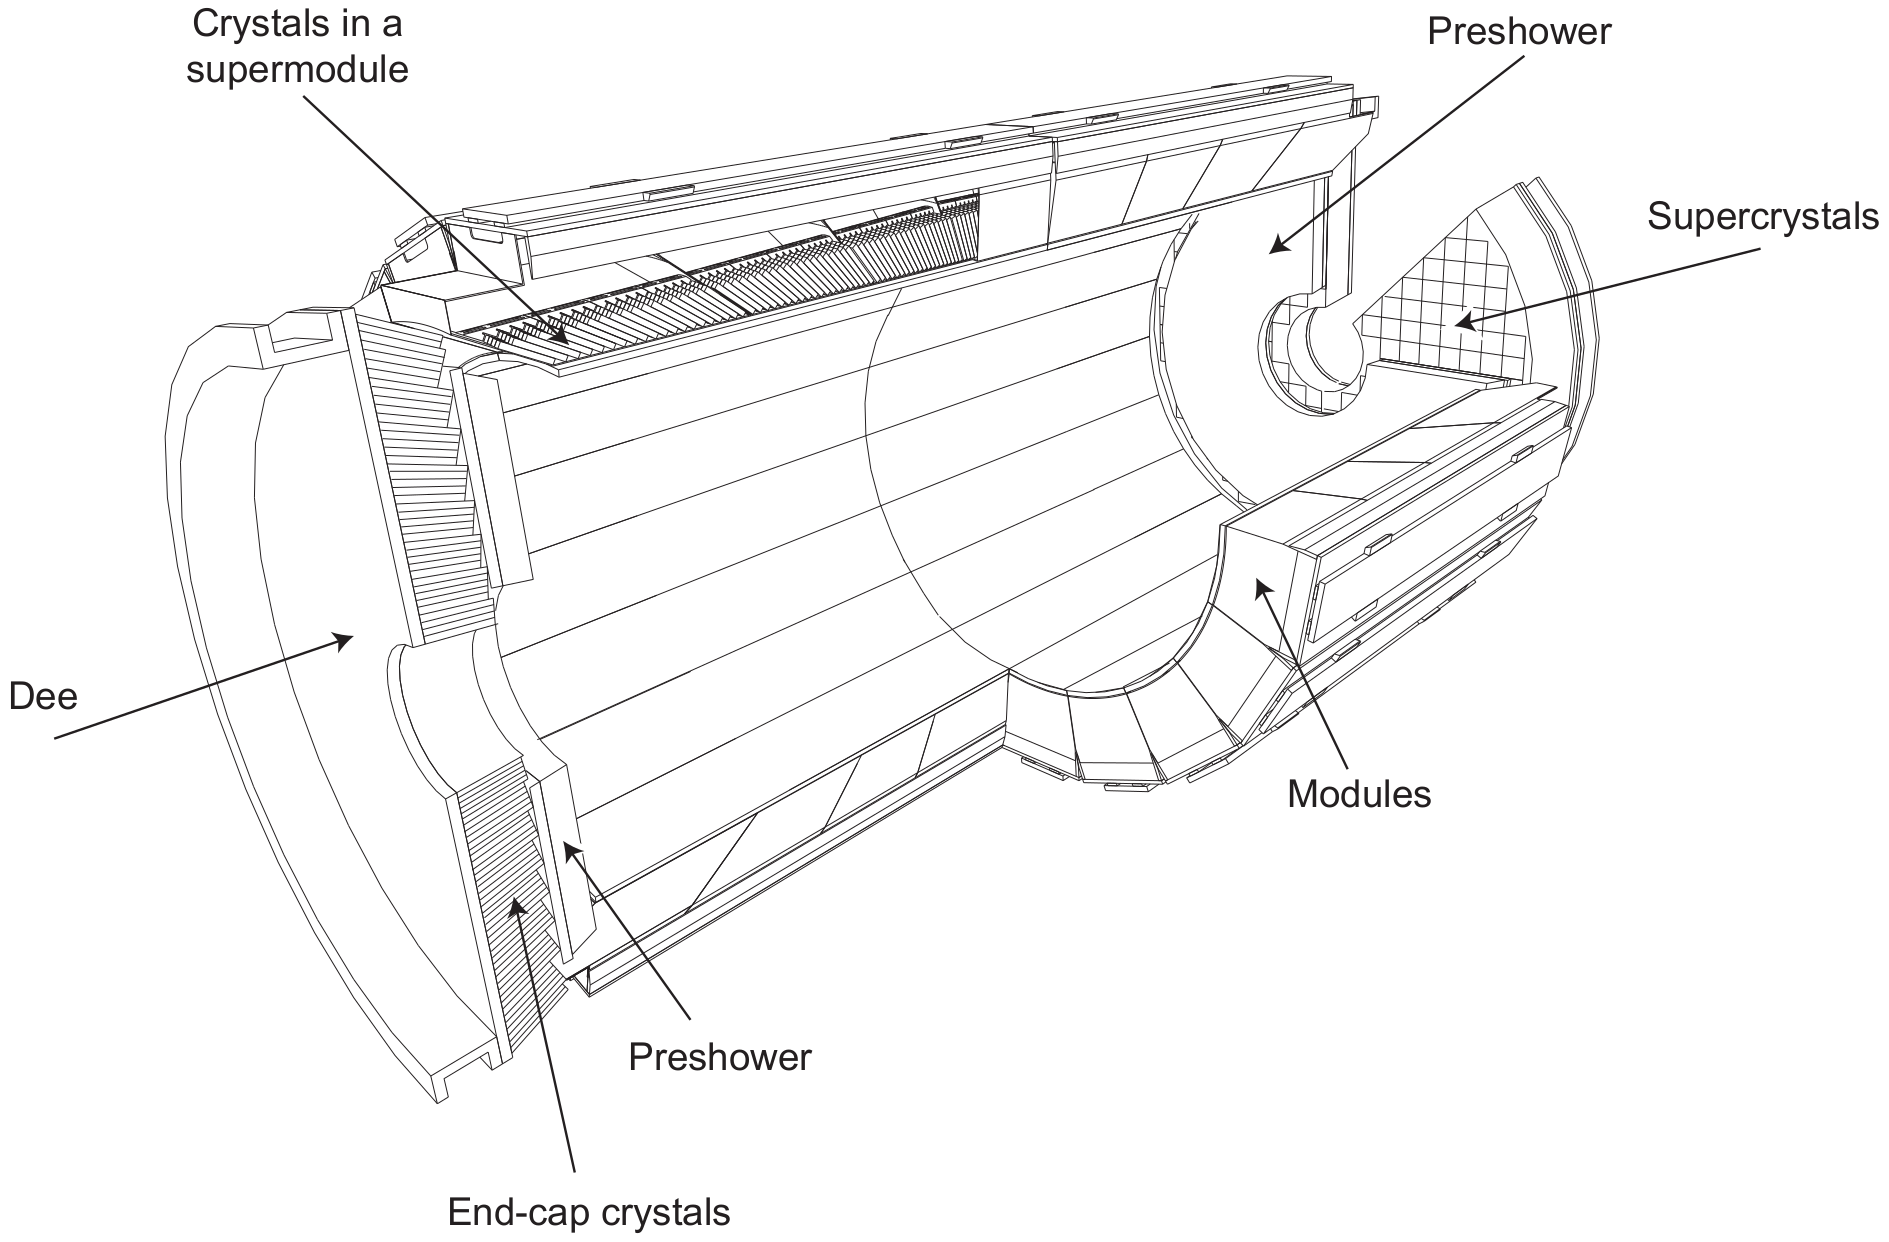
\includegraphics[width=0.8\textwidth]{ECAL-trans.png}
  \caption{Vue en perspective du calorimètre électromagnétique et de ses sous-éléments \cite{CMStechnical}.}
  \label{fig:ecaltrans}
\end{center}
\end{figure}


\subsubsection{Les cristaux}


Ces cristaux ont été spécialement conçus pour avoir une faible longueur de radiation\footnote{Longueur pour qu'un électron perde \sfrac{2}{3} de son énergie.} $X_0$, c'est-à-dire qu'ils sont capables de capter les photons et les électrons sur une distance relativement courte ($X_0 = \SI{0.89}{\cm}$).  
Le $PbWO_4$ possède également un faible rayon de molière (\SI{2.19}{\cm}) \footnote{Le rayon de Molière définit la taille du cylindre qui captera 90\% de l'énergie de la gerbe électromagnétique.}. On a également la possibilité d'utiliser des cristaux ayant des dimensions très réduites. Plus précisément, \SI{21.8}{\mm} $\times$ \SI{21.8}{\mm} de surface dans le tonneau, et \SI{24.7}{\mm} $\times$ \SI{24.7}{\mm} de surface dans les bouchons, ce qui implique une très grande granularité en $\eta$ et $\phi$ et donc la haute densité des cristaux ($\SI{8.29}{\g \per \cm\cubed}$).

Cependant, il existe un inconvénient majeur qu'est la forte sensibilité de la réponse à la température ($\SI{\sim 2}{\percent\per\degreeCelsius}$). Cela impose un système de refroidissement pour maintenir une température très stable dans le ECAL ($\pm \SI{0.05}{\degreeCelsius}$).

Lors du passage d'un électron ou d'un photon, de la lumière est émise en quantité proportionnelle à l'énergie déposée dans le cristal, il s'agit d'un phénomène de scintillation. Des photodétecteurs sont associés à chaque cristal pour capter cette lumière. Le champ magnétique intense de \SI{3.8}{\tesla} et les très fortes radiations ont imposé le choix de deux technologies différentes : les photodiodes à avalanches pour le tonneau (APD), et les phototriodes à vide pour les bouchons (VPT).

\subsubsection{Le détecteur à pied de gerbe}

A cause de la granularité insuffisante des cristaux dans les bouchons, certains hadrons neutres, tels que les $\pi^0$, se désintégrant en deux photons, peuvent être interprétés comme un photon par le calorimètre. 

Ainsi, pour faciliter la discrimination des photons issus d'évènements durs et ceux issus de la désintégration d'hadrons neutres, il a été décidé de placer un détecteur à pied de gerbe en amont du calorimètre électromagnétique, dans les bouchons.
Ce détecteur permet d'initier la gerbe électromagnétique avant d'entrer dans le ECAL, grâce à une plaque de plomb et d'aluminium. Couvrant une région en $\abs{\eta}$ entre \num{1.653} et \num{2.6}
%(voir figure \figurename{\ref{fig:ecal}}) 
avec une surface de détection en silicium de \SI{8}{\square\meter}, il possède une granularité bien plus importante que le ECAL, avec des bandes de détection de \SI{2}{\mm} de large. Grâce à ce dispositif, il est, par exemple, possible d'améliorer la distinction des photons issus d'un $\pi^0$ boosté.

%\begin{figure}
%\begin{center}
%  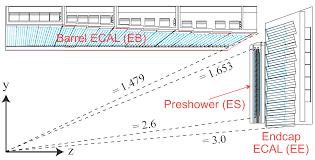
\includegraphics[width=0.7\textwidth]{ECAL.png}
%  \caption{Vue en coupe du calorimètre électromagnétique et de ses sous-éléments \cite{CMStechnical}.}
%  \label{fig:ecal}
%\end{center}
%\end{figure}

\begin{figure} 
\begin{center}
  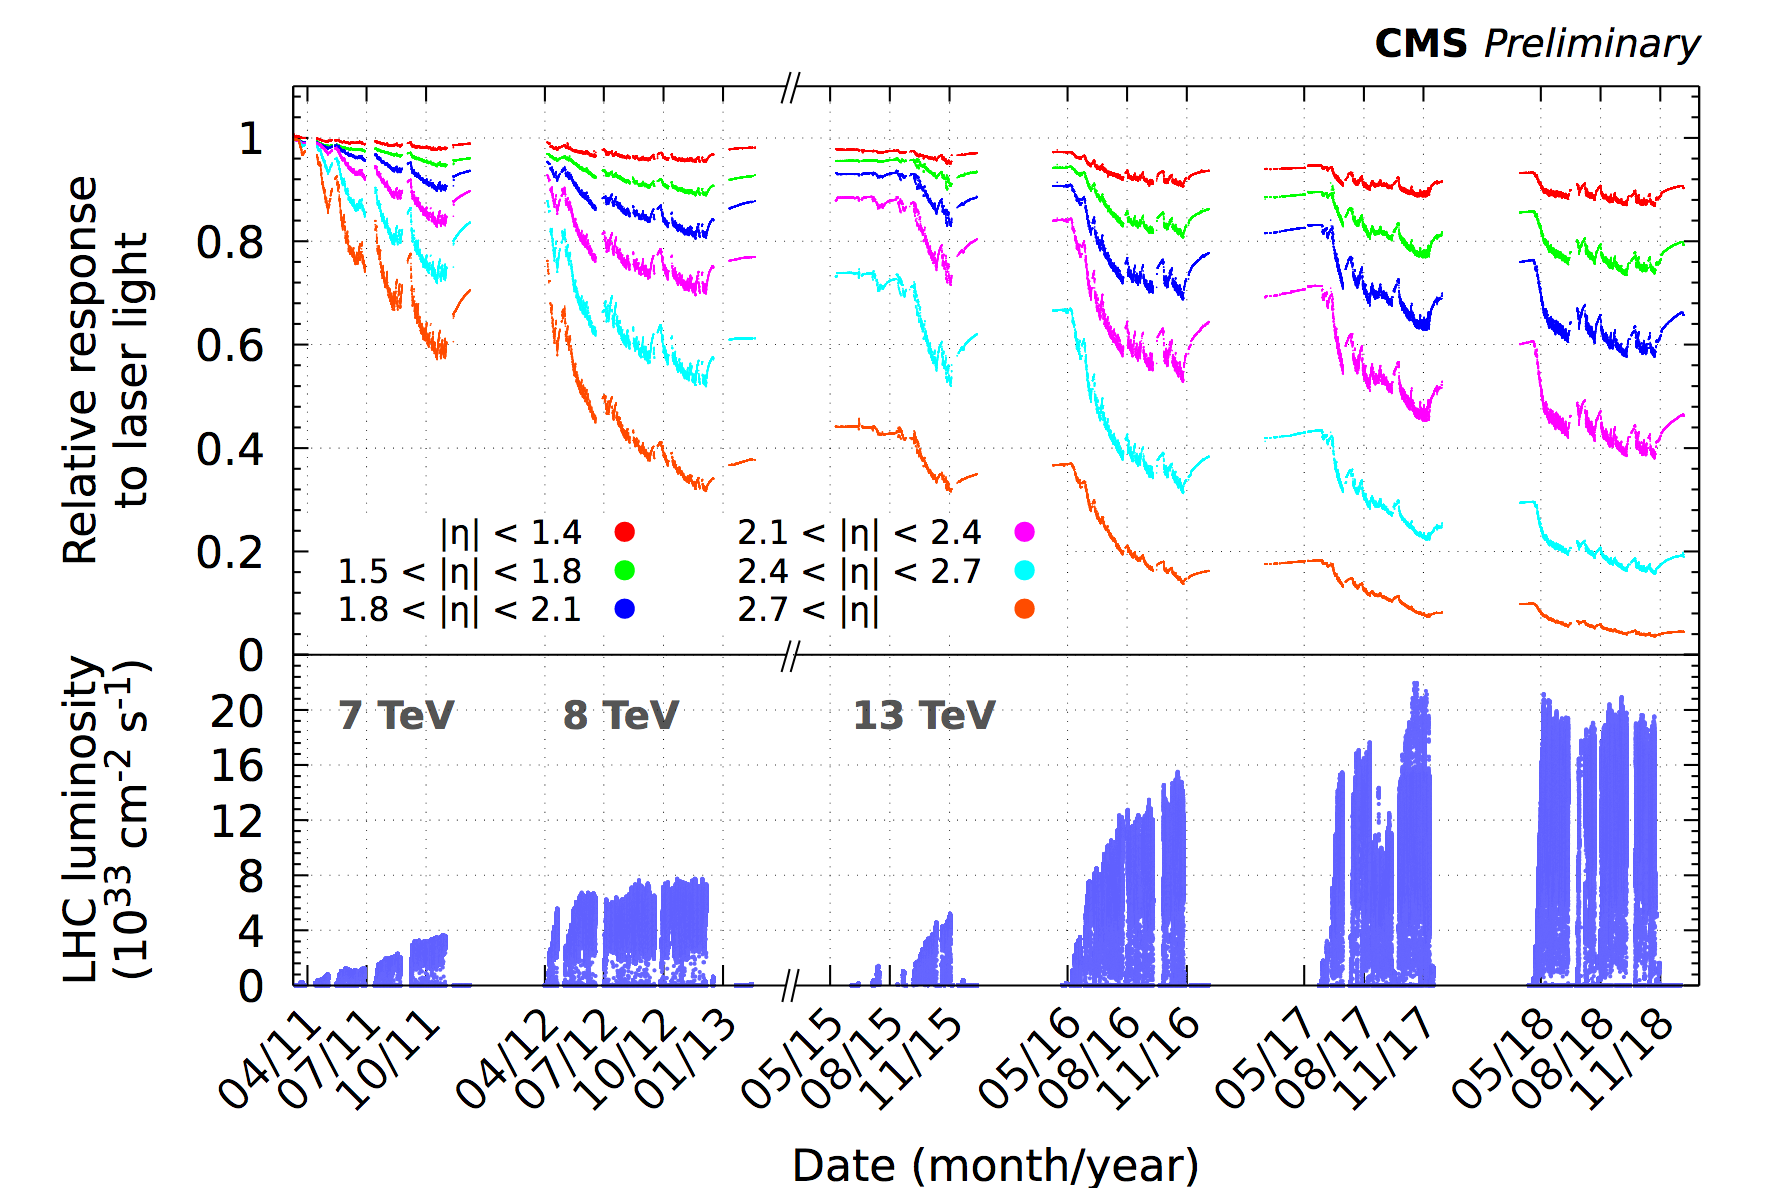
\includegraphics[width=0.9\textwidth]{ecal_transparency.png}
  \caption{Réponse relative des cristaux du ECAL en fonction du temps, pour différentes zones en \aeta (\emph{haut}) et luminosité instantanée du LHC (\emph{bas}) \cite{CMS-DP-2019-005}.}
  \label{fig:ecal_performance}
\end{center}
\end{figure}


\subsubsection{Performances}

\begin{figure}
\begin{center}
  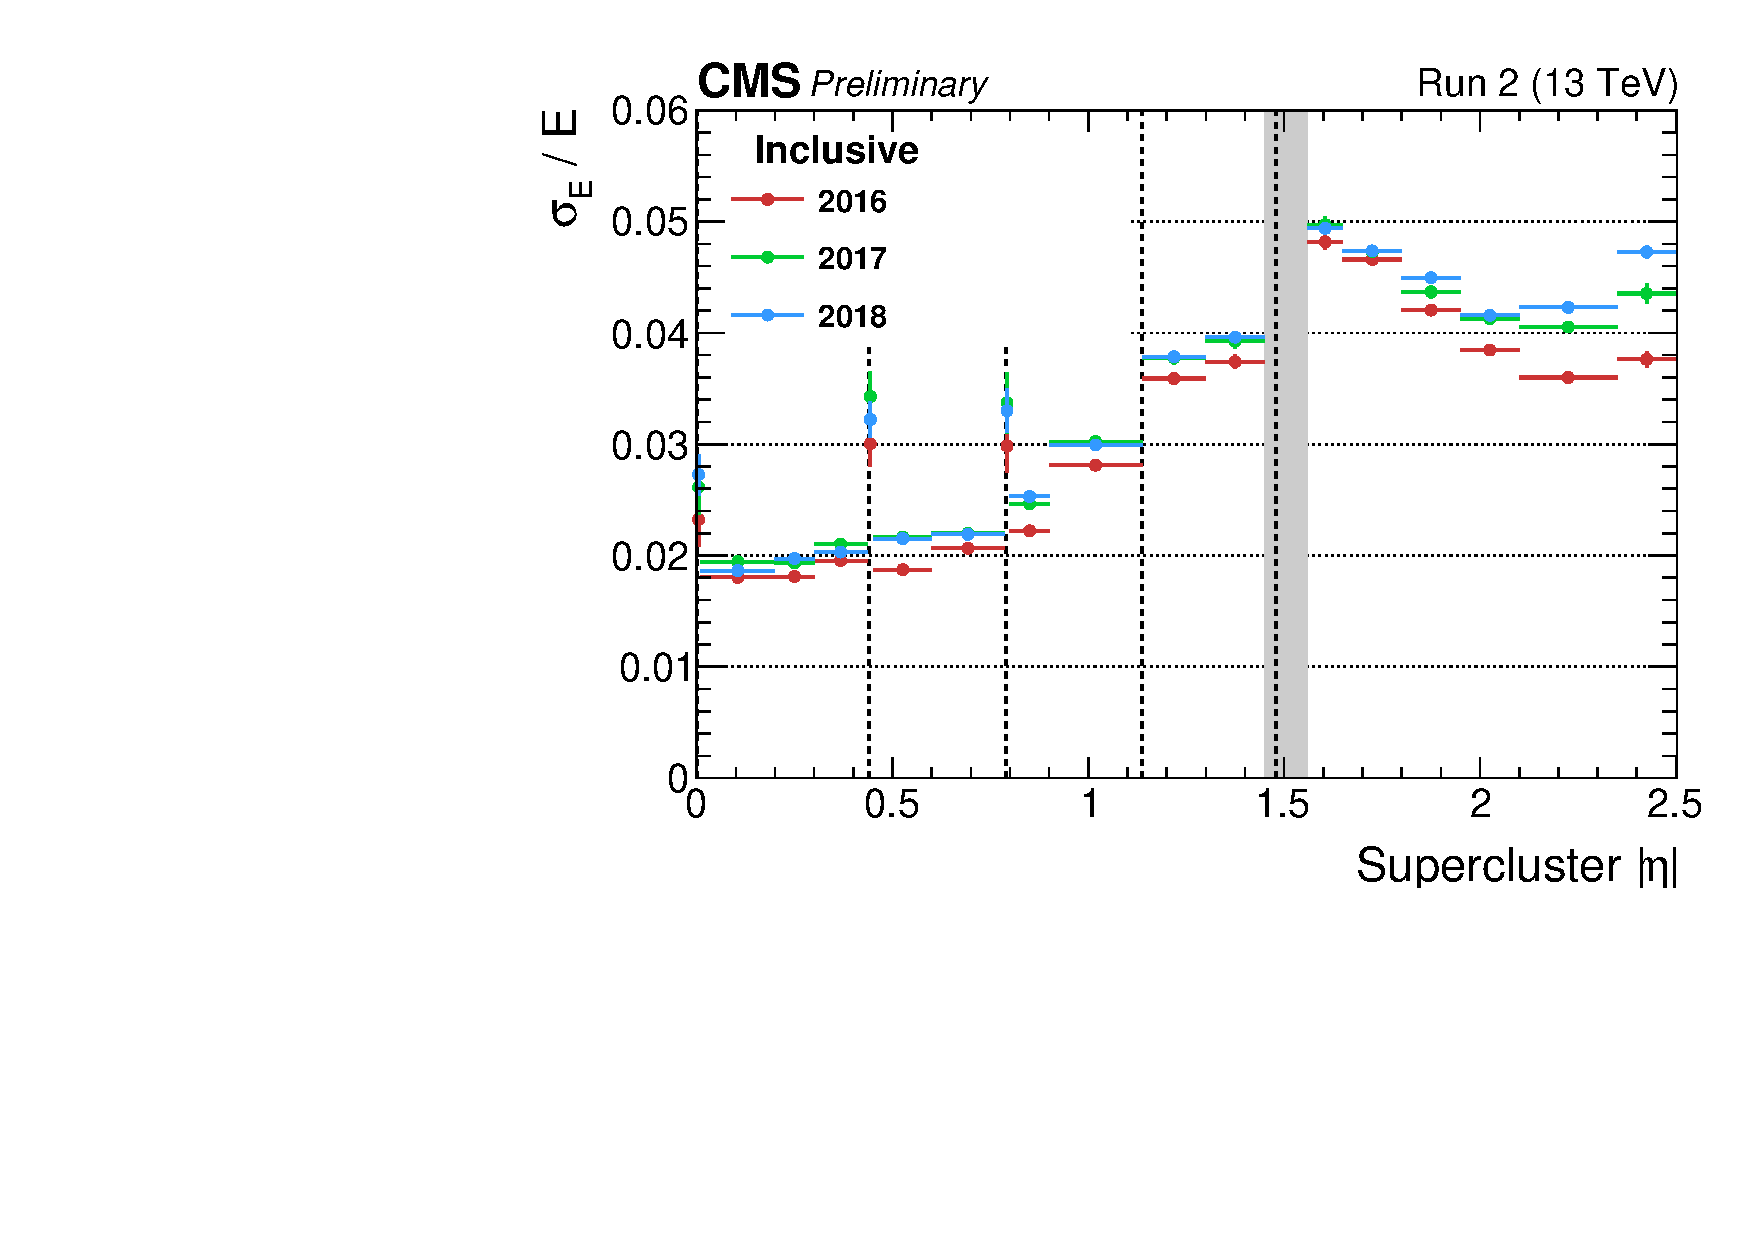
\includegraphics[width=0.6\textwidth,angle=-90]{EcalEnergyResolutionGolden.pdf}
  \caption{Résolution relative du ECAL lors du Run II en fonction de la position angulaire $\eta$ du super-cluster des électrons issus des désintégrations $\PZ \rightarrow \Pelectron \APelectron$ \cite{Mans:1481837}.}
  \label{fig:ecal_resolution}
\end{center}
\end{figure}

Une caractéristique impactant les cristaux du ECAL est la sensibilité aux radiations. Cette sensibilité se manifeste par la perte de transparence des cristaux au fil du temps. Afin de mesurer cet effet, un système de contrôle a été mis en place. Un balayage laser est envoyé sur tous les cristaux afin de mesurer leur transparence. On peut voir dans la figure \figurename{\ref{fig:ecal_performance}} la réponse relative des cristaux du ECAL en fonction de la date de prise de données. On constate clairement la diminution de la réponse relative. Des corrections sont déployées pour corriger cet effet. 


La résolution $\sigma$ du ECAL est paramétrée par :
\begin{align*}
  \left( \frac{\sigma}{E} \right)^2 &= \left( \frac{S}{\sqrt{E}} \right)^2 + \left( \frac{N}{E} \right)^2 + C^2
\end{align*}
où $S$ est le terme stochastique, dû aux fluctuations dans l'étalement latéral de la gerbe électronique, $N$ le terme de bruit des composants électroniques, et $C$ un terme constant qui prend en compte les erreurs de calibration.
On peut voir figure \figurename{\ref{fig:ecal_resolution}} l'évolution de la résolution relative en fonction de la position angulaire $\eta$ du super-cluster d'énergie.
La paramétrisation, lors de tests sur faisceaux en 2006, fut évaluée à
\begin{align*}
  \left( \frac{\sigma}{E} \right)^2 &= \left( \frac{\SI{2.8}{\%}}{\sqrt{E}} \right)^2 + \left( \frac{\num{0.12}}{E} \right)^2 + \left(\SI{0.30}{\%}\right)^2
\end{align*}

\subsection{Calorimètre hadronique}


Le calorimètre hadronique (HCAL, pour \emph{Hadronic CALorimeter}) permet de mesurer l'énergie des hadrons neutres et chargés. Une succession de couches d'absorbants et de scintillateurs permet de déterminer la trajectoire et l'énergie d'une particule incidente. Il est constitué de trois parties : une partie tonneaux (HB et HO) et bouchon (HE) de manière analogue aux ECAL et une partie périphérique au détecteur (HF). Une vue longitudinale du HCAL est visible à la figure \figurename{\ref{fig:hcal}}. Il est à noter que le HCAL est impliqué également dans le déclenchement (voir section \ref{declenchement}).


\begin{figure}
\begin{center}
  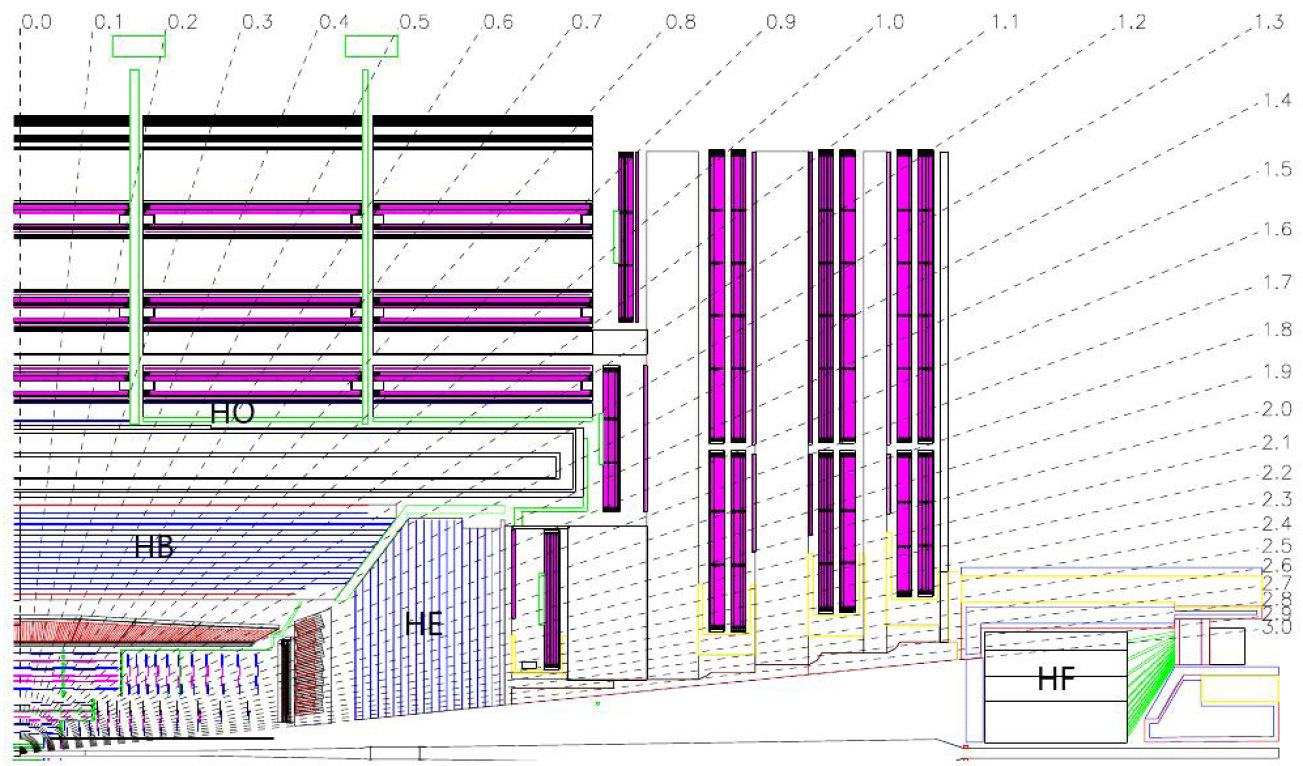
\includegraphics[width=0.7\textwidth]{HCAL.png}
  \caption{Vue longitudinale du calorimètre hadronique \cite{CMStechnical}.}
  \label{fig:hcal}
\end{center}
\end{figure}

Pour comprendre les caractéristiques intrinsèques du HCAL on définit la longueur d'interaction nucléaire $\lambda_0$. Caractéristique des matériaux, elle est la longueur après laquelle \SI{36.8}{\%} ($\sfrac{1}{e}$) des hadrons seront absorbés par le milieu. L'absorbant retenu pour le tonneau et les bouchons du HCAL est le laiton avec $\lambda_0 = \SI{16.42}{\cm}$.
Cet alliage a été choisi pour ses propriétés paramagnétiques, dues au placement du HCAL à l'intérieur de l'aimant. Le laiton est également quasi transparent pour les muons, ce qui permet de conserver la quasi totalité de leur impulsion en traversant le détecteur. Chaque couche d'absorbant mesure \SI{5}{\cm} d'épaisseur dans le tonneau, et \SI{8}{\cm} dans les bouchons. Entre chaque couche d'absorbant se trouve une couche de scintillateur plastique de \SI{3.7}{\mm} d'épaisseur. 

Le tonneau couvre une zone angulaire entre $0 \leq \abs{\eta} < \num{1.48}$, et est composé de deux parties différentes. La première partie, le HB, mesure \SI{89}{\cm} de profondeur, soit seulement \SI{5.82}{\lambda_0}. Cette longueur est insuffisante pour absorber la totalité de la gerbe hadronique. Une deuxième partie, le HO, a donc été ajoutée, située à l'extérieur du solénoïde. L'aimant sert alors d'absorbeur, et le HO détecte les gerbes longues ou tardives. Les bouchons couvrent une zone angulaire entre $1.48 \leq \abs{\eta} < \num{3}$. La longueur totale du calorimètre est, en incluant le ECAL, d'environ \SI{10}{\lambda_0}, suffisante pour arrêter la gerbe hadronique.

La dernière partie, le HF, couvre une zone angulaire entre $\num{2.9} \leq \abs{\eta} < \num{5.2}$. C'est un cylindre de \SI{130}{\cm} de rayon, situé à \SI{11.2}{\m} du point d'interaction. D'une longueur de \SI{165}{\cm} (\SI{\sim 10}{\lambda_0}), il est constitué d'un absorbeur en acier, dans lequel sont introduites des fibres optiques en quartz. Les particules chargées entrant dans le milieu émettent des photons par effet Cherenkov. Ils sont collectés par les fibres puis amplifiés par photomultiplicateurs.

Les premières études du HCAL ont évalué, après calibration \cite{Elvira:800406}, les résolutions en énergie à \SI{10}{\%} (HE), \SI{12}{\%} (HF) et \SI{5}{\%} (HO).


\subsection{Chambres à muons}



Le détecteur à muons joue un rôle central dans CMS, puisqu'il couvre trois fonctions principales : identifier les muons, mesurer leur impulsion, et assurer une partie du déclenchement (voir \ref{declenchement}). Il s'agit de la partie externe du détecteur. Les autres types de particules ayant déjà déposé leur énergie dans les autres sous-détecteurs de CMS, seuls les muons pourront l'atteindre. Son éloignement au trajectographe, rend la mesure de l'impulsion de ces particules beaucoup plus facile avec leur temps de vie de  \SI{2,2}{\micro\second}.


\begin{figure}
\begin{center}
  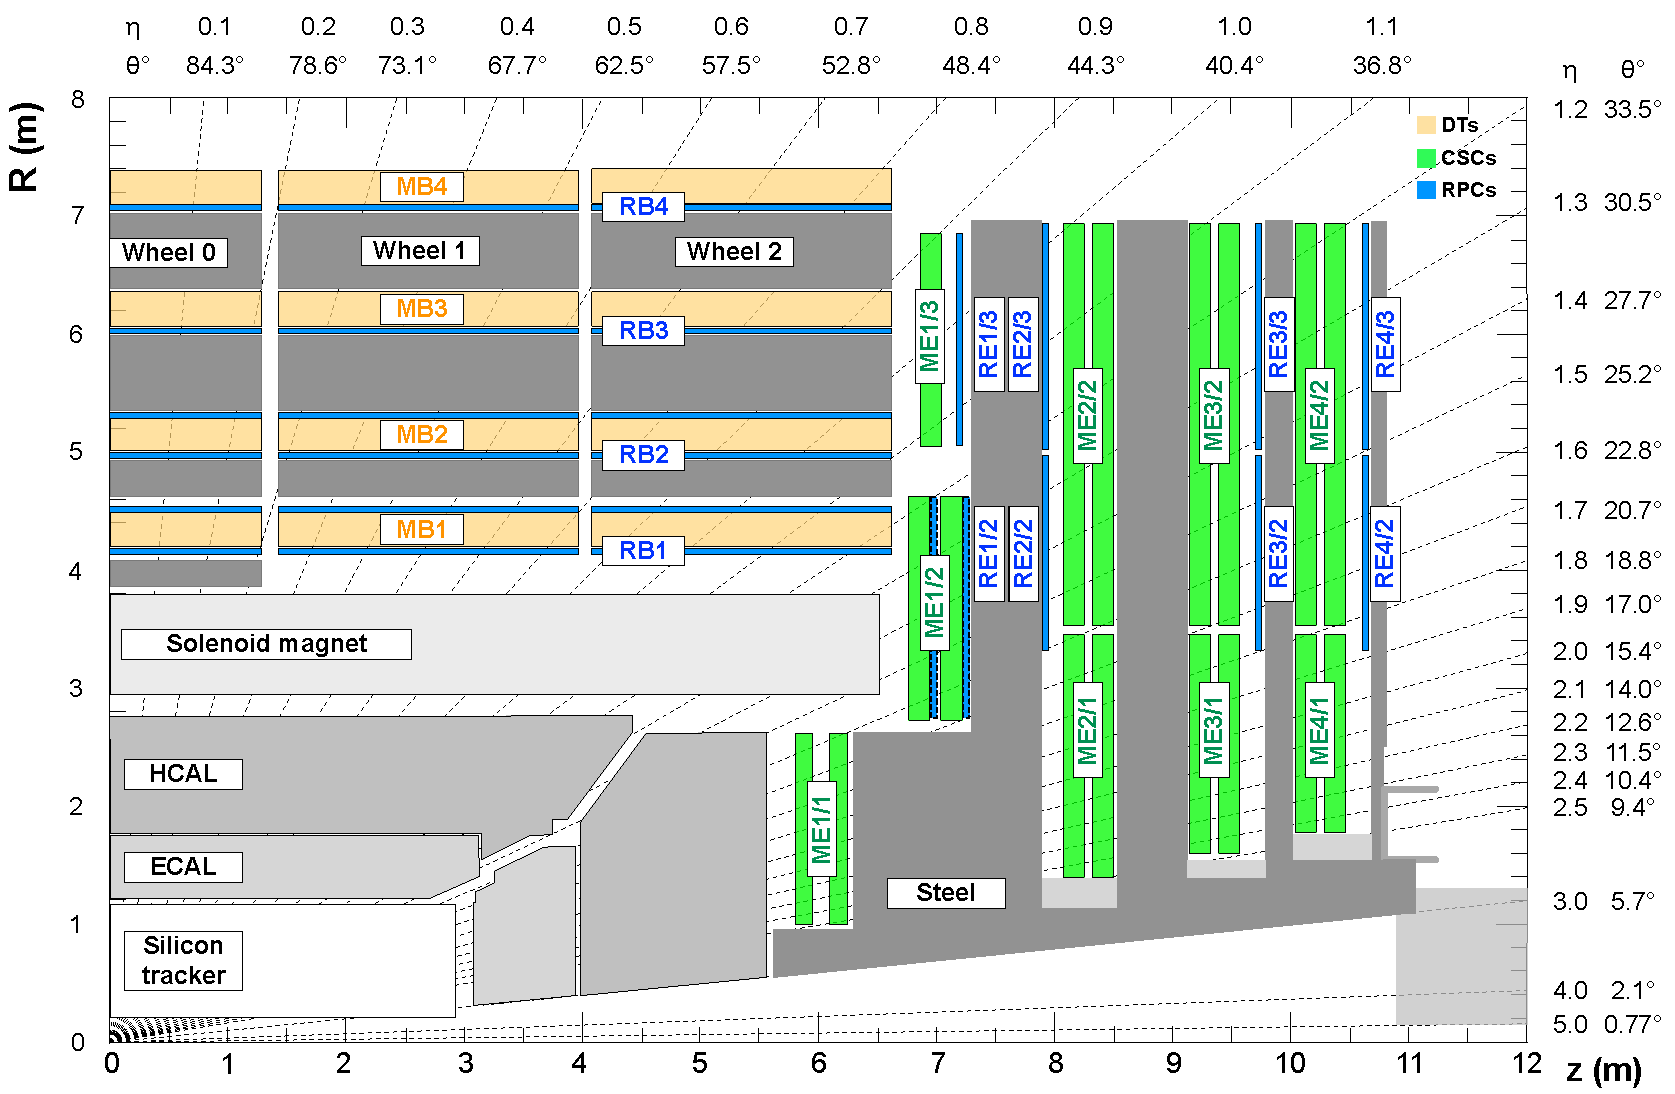
\includegraphics[width=0.7\textwidth]{muonchamber.pdf}
  \caption{Vue longitudinale des chambres à muons \cite{CMStechnical}.}
  \label{fig:cms_csc}
\end{center}
\end{figure}

Il existe trois types de détecteurs à gaz différents dans les chambres, dont l'agencement est présenté sur la figure \figurename{\ref{fig:cms_csc}}.

\begin{figure} \centering
  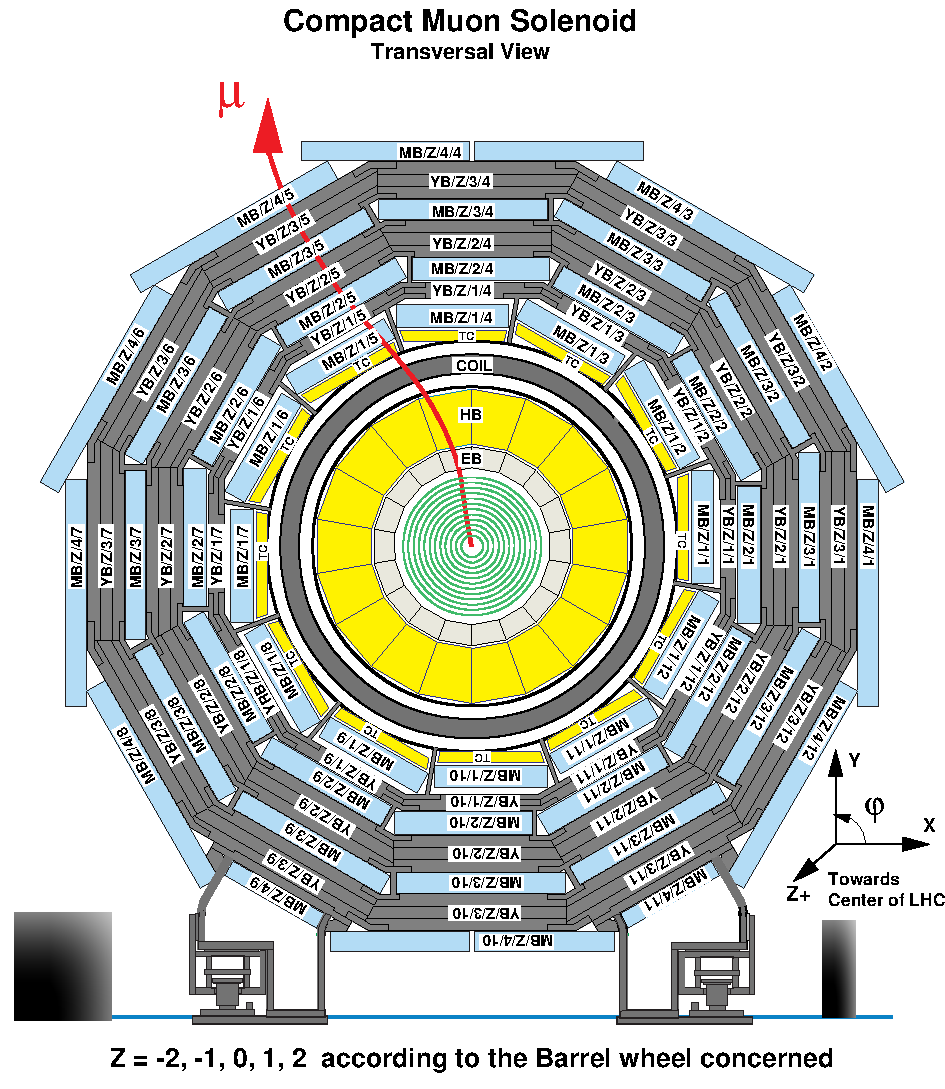
\includegraphics[width=0.8\textwidth]{CMS_transverse_view.pdf}
  \caption{Agencement des tubes à dérives dans le tonneau de CMS (vue transverse). Chaque rectangle bleu correspond à un tube à dérive.}
  \label{fig:cms_dt}
\end{figure}


\begin{description}
  \item[Les tubes à dérive (DT)] Installés dans le tonneau (voir figure \figurename{\ref{fig:cms_dt}}), ils couvrent une zone angulaire $\abs{\eta} < 1.2$. Il y a 250 stations de DT dans le détecteur.
  \item[Les chambres à pistes cathodiques (CSC)] Installées dans les bouchons, elles sont conçues pour supporter les variations du champ magnétique et les fortes radiations. 540 de ces modules sont installés, sur une zone angulaire $\num{0.9} < \abs{\eta} < \num{2.4}$.
  \item[Les détecteurs à plaques résistives (RPC)] Installés à la fois dans le tonneau et dans les bouchons, ils permettent d'assurer une partie du déclenchement grâce à leur temps de réponse inférieur à \SI{25}{\ns}.
\end{description}


\subsection{Système de déclenchement}
\label{declenchement}
\begin{figure}
\begin{center}
  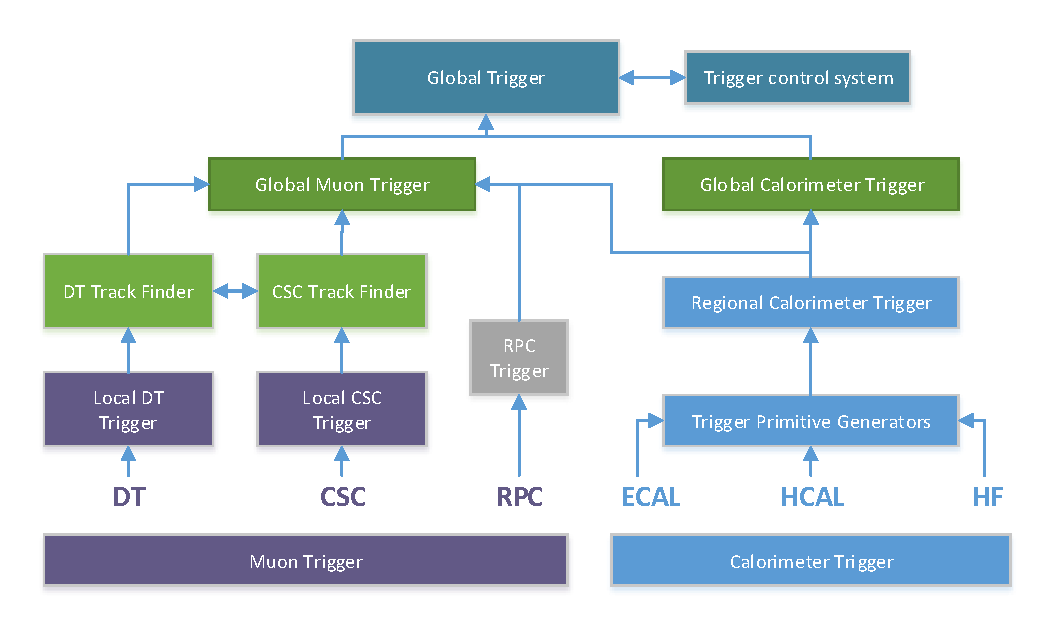
\includegraphics[width=0.7\textwidth]{L1.pdf}
  \caption{L'architecture du déclencheur de niveau 1}
  \label{fig:l1}
\end{center}
\end{figure}

Pendant une prise de données, les paquets de protons se croisent toutes les \SI{25}{\ns}, soit une fréquence de collisions de \SI{40}{\mega\hertz}. Or seul un flux de \SI{\sim 0.4}{\giga\octet\per\second} peut être enregistré sur disque. 
En estimant un événement à environ \SI{2}{\mega\octet}, on obtient alors un débit de données de \SI{80}{\tera\octet\per\second}, bien trop élevé pour être traité en temps réel. La stratégie est de sélectionner en ligne les évènements que l'on veut garder et ignorer ceux qui présentent peu d'intérêt pour les analyses de la collaboration.

Pour cela, on utilise un système de déclenchement (\emph{trigger}), à deux niveaux : le niveau 1 (L1) et le HLT (\emph{High Level Trigger}, pour déclenchement de haut niveau). Les figures  \figurename{\ref{fig:l1}} et \figurename{\ref{fig:daq}} présentent respectivement l'architecture des déclenchements L1 et HLT. 

\begin{description}
  \item[Le L1] En utilisant directement les informations provenant du détecteur à muons et des calorimètres, ce premier niveau de déclenchement réduit le taux d’événements de \SI{40}{\mega\hertz} à \SI{100}{\kHz}. La décision de garder ou non l'événement est prise en moins de \SI{3.2}{\us}. Cette structure électronique gère 128 algorithmes de déclenchement tournant en parallèle.
  \item[Le HLT] Le taux d'événements doit être réduit à environ \SI{100}{\Hz} \cite{CMStrigger} afin d'être enregistré en temps réel. Les HLT, chargés d'effectuer cette sélection, utilisent une ferme d'ordinateurs, installée à proximité du détecteur. Cette ferme réalise une reconstruction rapide afin d'obtenir une description de l'événement en terme d'objets physiques (photon, muon, électrons et jets). Les conditions de sélections sont hautement configurables (choix des particules présentes, seuil en énergie, ...) ainsi de nombreux HLT différents sont utilisés. Le temps moyen alloué au HLT pour prendre une décision est d'environ \SI{50}{\ms}. 
\end{description}

Une fois accepté, l'événement est stocké de façon définitive dans un centre de stockage à haute redondance, le \emph{Tier-0}.

\begin{figure}
\begin{center}
  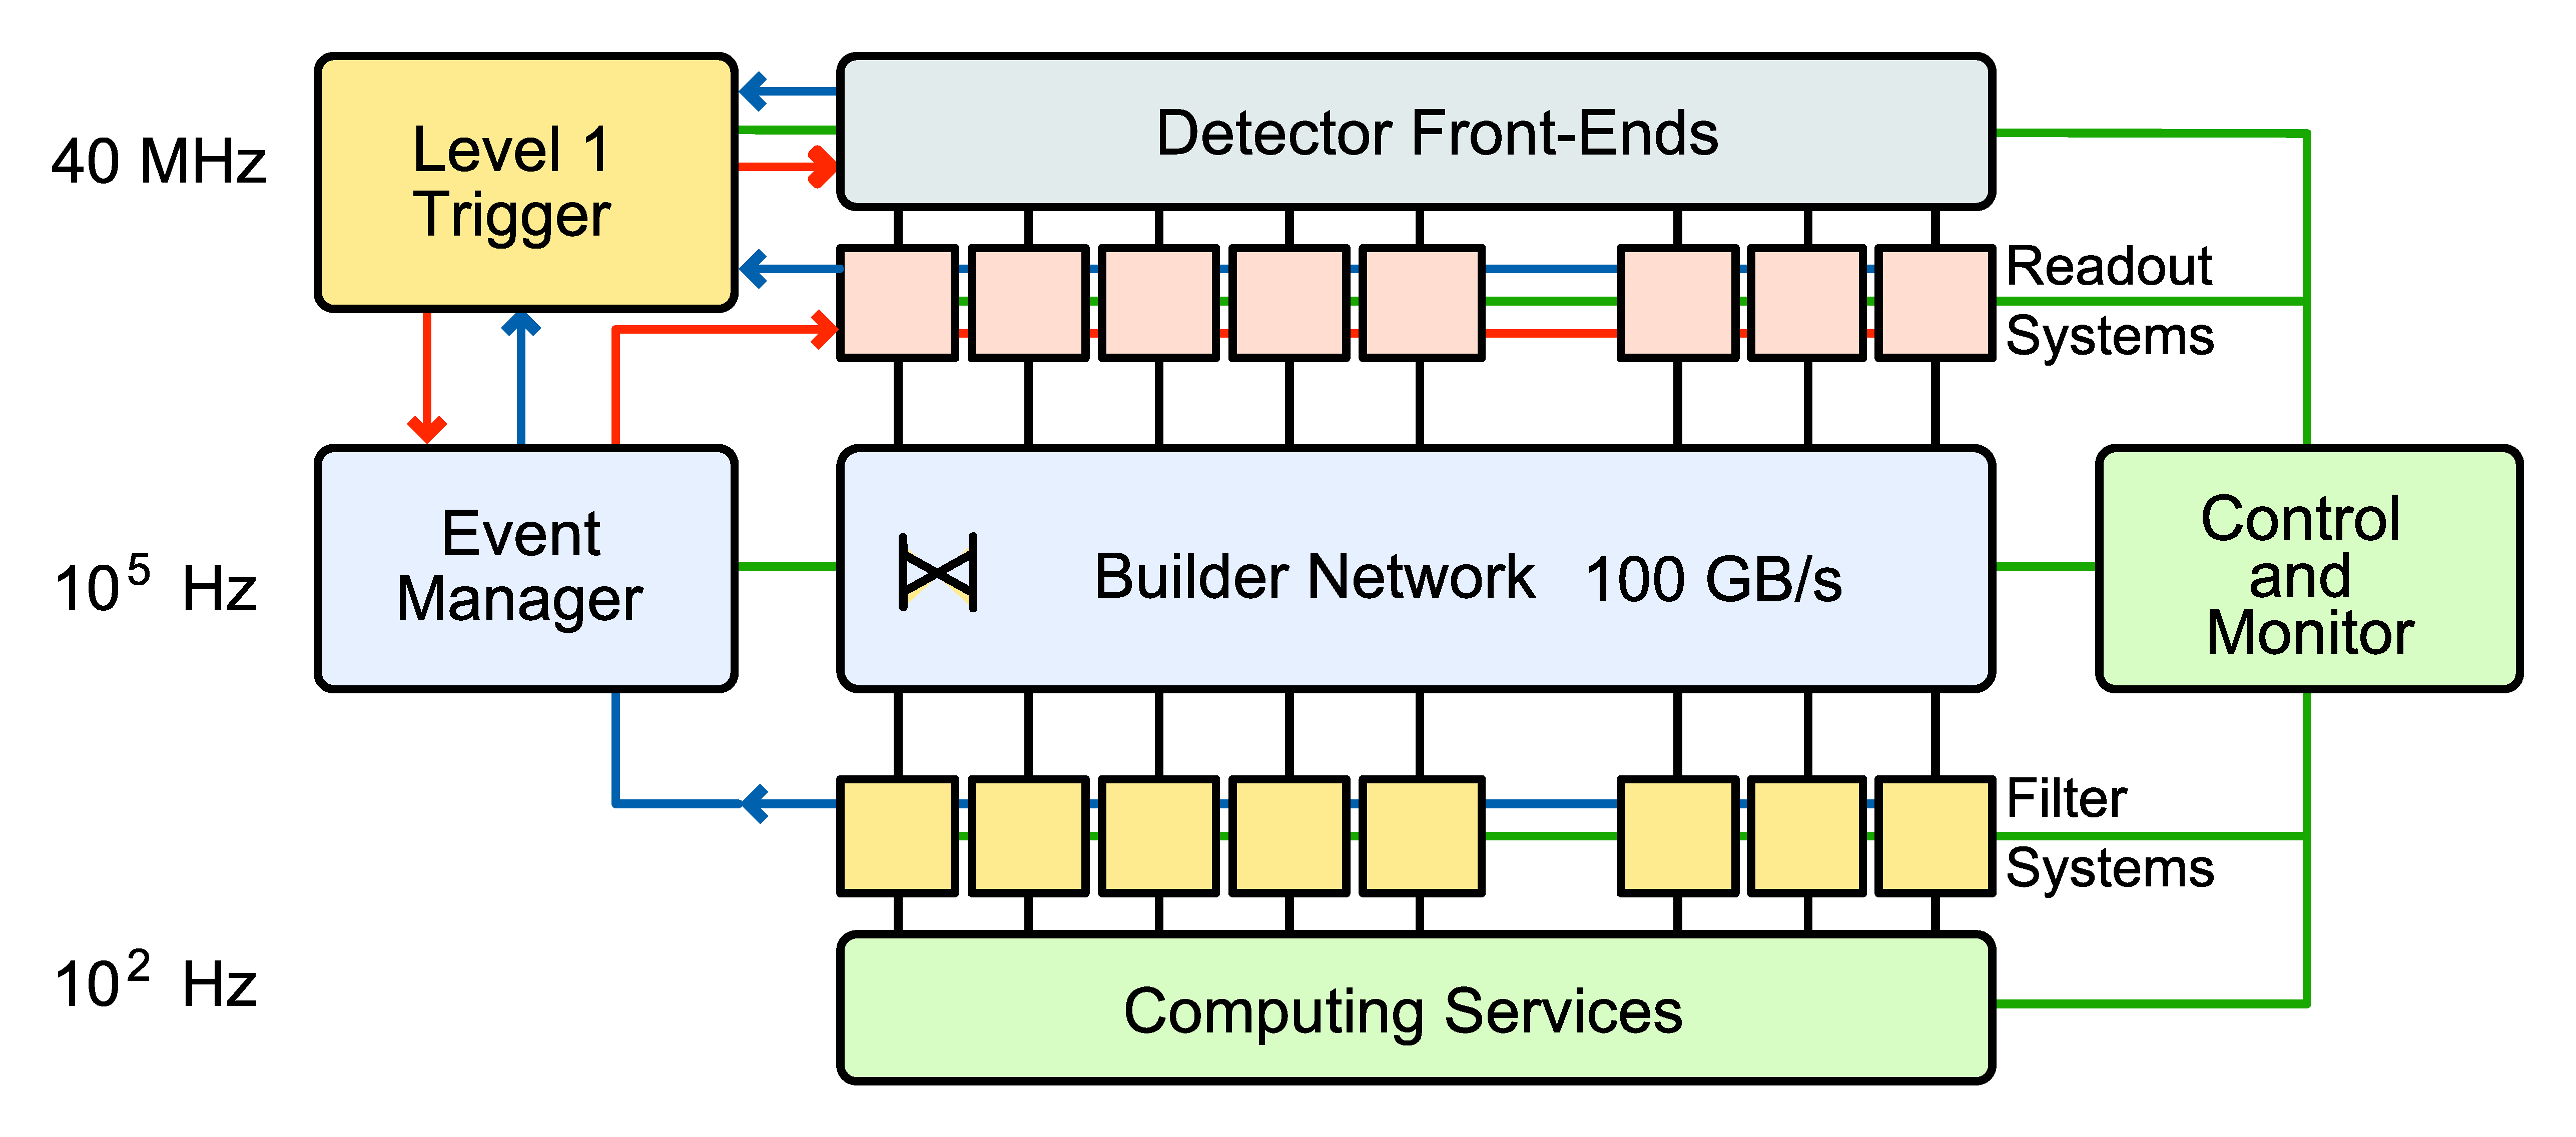
\includegraphics[width=0.7\textwidth]{DAQ.pdf}
  \caption{Schéma de la chaîne d'acquisition de données de CMS}
  \label{fig:daq}
\end{center}
\end{figure}



\section{Mesure de la luminosité}\label{sec:luminosity}

La mesure de la luminosité est un aspect important pour les analyses physiques. Pour l'analyse contenue dans cette thèse, la compréhension de cette mesure est d'autant plus importante qu'elle est à la fois l'incertitude systématique dominante mais également une quantité corrélée au temps.
A CMS la luminosité est mesurée avec une combinaison de cinq luminomètres principaux :
\begin{description}
\item[Pixel Luminosity Telescope (PLT)] 
\begin{sloppypar}
Il s'agit d'un sous-détecteur dédié à la mesure de la luminosité en utilisant des capteurs en pixel de silicium. Les quarante-huit capteurs sont répartis en seize piles de trois capteurs appelées "télescopes". Le PLT mesure le taux de "triples mesures", c'est-à-dire le taux de signaux enregistrés sur les trois capteurs d'un même télescope.
\end{sloppypar}
\item[Fast Beam Conditions Monitor (BCM1F)] 
\begin{sloppypar}
Ce sous-détecteur est composé de dix capteurs en silicium, dix capteurs en diamant polycristallins (pCVD) et quatre capteurs en diamant monocristal (sCVD). Cette structure est dotée d'une lecture rapide à \SI{6.25}{\nano\second} qui permet l'enregistrement de la luminosité en temps réel.
\end{sloppypar}
\item[Forward Calorimeter (HF)] 
\begin{sloppypar}
Le HF joue un rôle clé dans CMS puisqu'il permet de mesurer en temps réel la luminosité instantanée reçue par CMS. Deux méthodes sont utilisées. La première utilise le nombre de tours sans signal pour en déduire le nombre moyen d'interactions par croisements de faisceaux. La deuxième méthode tire parti de la relation linéaire qui existe entre l'énergie transverse moyenne par tour et la luminosité.
\end{sloppypar}
\item[Pixel Detector] 
\begin{sloppypar}
Ce détecteur à pixels contient \num{65e6} pixels, ce qui lui permet de mesurer les trajectoires des particules issues de la collision avec une extrême précision. C'est également le détecteur le plus proche du faisceau. Il est essentiel pour reconstruire les trajectoires des particules à très courte durée de vie.
\end{sloppypar}
\item[RAMSES]
\begin{sloppypar}
Depuis 2017, ce sous-détecteur fait partie des systèmes de protection et de surveillance de l'environnement du LHC, mais peut également être utilisé pour fournir une mesure de luminosité. Le capteur est une chambre d'ionisation cylindrique en plastique remplie de \SI{3}{\L} d'air à pression atmosphérique. Les parois sont recouvertes de \SI{4}{\mm} de graphite PE. Il détecte principalement les photons dans la gamme d'énergie de \SI{50}{\keV} à \SI{7}{\MeV}.
\end{sloppypar}
\end{description}

Afin de calibrer les méthodes de détections, le LHC effectue régulièrement des scans Van Der Meer \cite{Balagura_2021} pilotés par l'équation :
\begin{equation}
\sigma = \iint \frac{\mu(\Delta x, \Delta y)}{N_1 N_2}\mathrm{d}\Delta x \mathrm{d}\Delta y
\end{equation}
avec $\sigma $ la section efficace visible, $N_1$ et $N_2$ le nombre de protons dans chaque faisceau. L'intégrande est donné par :
\begin{equation}
\frac{\mu(\Delta x, \Delta y)}{N_1 N_2} = \sigma \frac{\mathcal{L}_\mathrm{inst}}{N_1 N_2}
\end{equation}
avec $\mathcal{L}_\mathrm{inst}$ la luminosité instantanée. En pratique, les scans permettent de déterminer précisément la forme horizontale et verticale des faisceaux, en décalant l'un des faisceaux selon l'axe $x$ ou $y$. Ils permettent en plus de déterminer la section efficace inélastique \Pproton{}\Pproton{} visible par les luminomètres ce qui permet de calibrer les mesures de luminosité.
\newline

Durant ma thèse, j'ai contribué à la calibration de la luminosité enregistrée en 2018, avec étude de l'incertitude sur le bruit de fond du détecteur. Nous avons utilisé la méthode du comptage d'agrégats de pixels (ou PCC pour \emph{Pixel Cluster Counting}). Cette méthode consiste simplement en un décompte du nombre de clusters de pixels activés au passage d'une particule. 

Pour estimer le bruit de fond, il faut effectuer un PCC sur une zone temporelle d'arrêt de l'activité du LHC. Cette zone est identifiable car elle consiste en une longue pause entre deux scans Van Der Meer. L'étude s'est portée sur deux scans à longues séparations effectués le 30 juin et le 1er juillet 2018 où les deux faisceaux étaient séparés par une distance de \SI{6}{\sigma}, où $\sigma$ est la largeur du paquet de protons. Le nombre moyen de clusters est mesuré à $ \langle n_\textrm{cluster}  \rangle = 0.169  \SI{\pm  0.003}{(stat)}$.
\newline

J'ai proposé une incertitude systématique, en examinant la variation du nombre moyen de clusters en fonction du temps, en utilisant les deux scans à longues séparations. Ce procédé a révélé une stabilité contenue dans l'incertitude systématique absolue de  $\sigma_\textrm{syst} = \num 0.010$ et visible dans la figure \figurename{\ref{fig:systematicFB}}.

\begin{figure}
\begin{center}
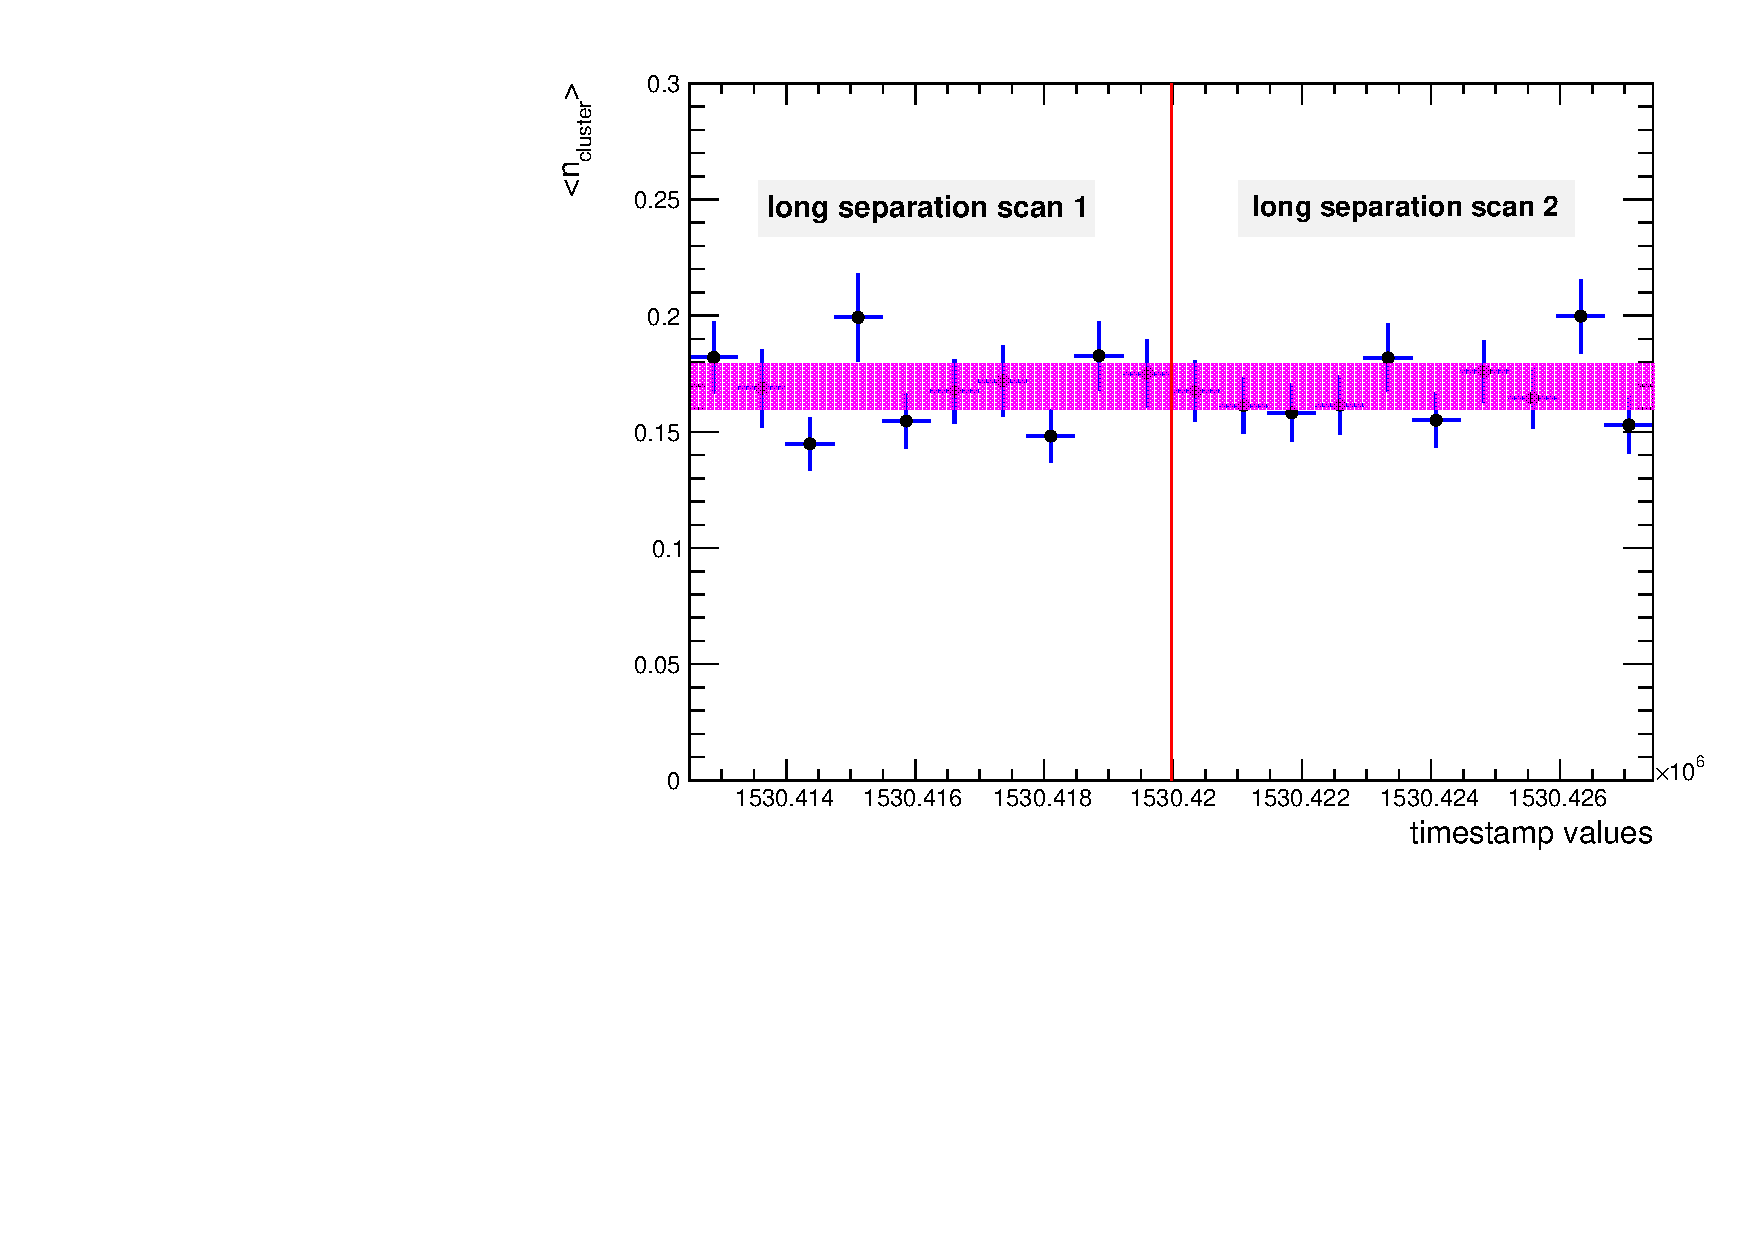
\includegraphics[width=0.5\textwidth, angle=-90]{systematicFB.pdf}
\end{center}
\caption{Incertitude systématique du comptage de clusters de pixels avec  $ \langle n_\textrm{cluster}  \rangle$ en fonction du temps, pour les deux scans à longue séparation.}
\label{fig:systematicFB}
\end{figure}

Le bruit de fond estimé par PCC est de 
\begin{equation}
 \langle n_\textrm{cluster}  \rangle  = 0.169 \SI{\pm  0.011}{(stat+syst)}
\end{equation}
où l'incertitude totale a été estimée par sommation en quadrature.

Des mesures similaires des bruits de fond sont effectuées avec les autres luminomètres par le groupe Luminosité de CMS. Ces mesures permettent de soustraire le taux de bruit de fond dans l'estimation des sections efficaces visibles, et sont donc importantes pour la calibration. Cette étude a contribué à la note publique de CMS \cite{CMS-PAS-LUM-18-002} pour l'estimation de la luminosité sur les données de 2018.
%été incluse dans la note d'analyse \cite{AN-2018/228} et

\section*{Conclusion}

Lors de ce chapitre, ont été présentés le LHC et le détecteur CMS. Leur conception a pour but d'enrichir nos connaissances du Modèle Standard grâce à des mesures de précision et d'offrir de nouvelles perspectives de recherche de nouvelles physiques au-delà Modèle Standard.
Pour assurer une analyse physique fonctionnelle, la première étape est la reconstruction des évènements d'une collision. Il s'agit de la transformation de signaux électriques captés par les différents sous-détecteurs de CMS en particules et autres objets physiques tels que des électrons, des muons et des gerbes hadroniques. Les méthodes utilisées par CMS sont décrites plus en détail dans le chapitre suivant.


\end{fmffile}
